% :vim:set sw=3:
\newcommand{\linksize}{\scriptsize}
%\newcommand{\textrightarrow}{$\,\to\,$}
\begin{document}

\begin{frame}[plain]
  \titlepage
\end{frame}

\begin{frame}
  \frametitle{Antonín Houska}

  \begin{columns}
    \begin{column}{0.8\textwidth}
      \begin{itemize}
	\item Antonín Houska, \href{mailto:ah@cybertec.at}{ah@cybertec.at}
	\item Postgres contributor since 2012
	\item Working as a Postgres developer for CYBERTEC since 2012
      \end{itemize}
    \end{column}
    \begin{column}{0.2\textwidth}
      \begin{center}
      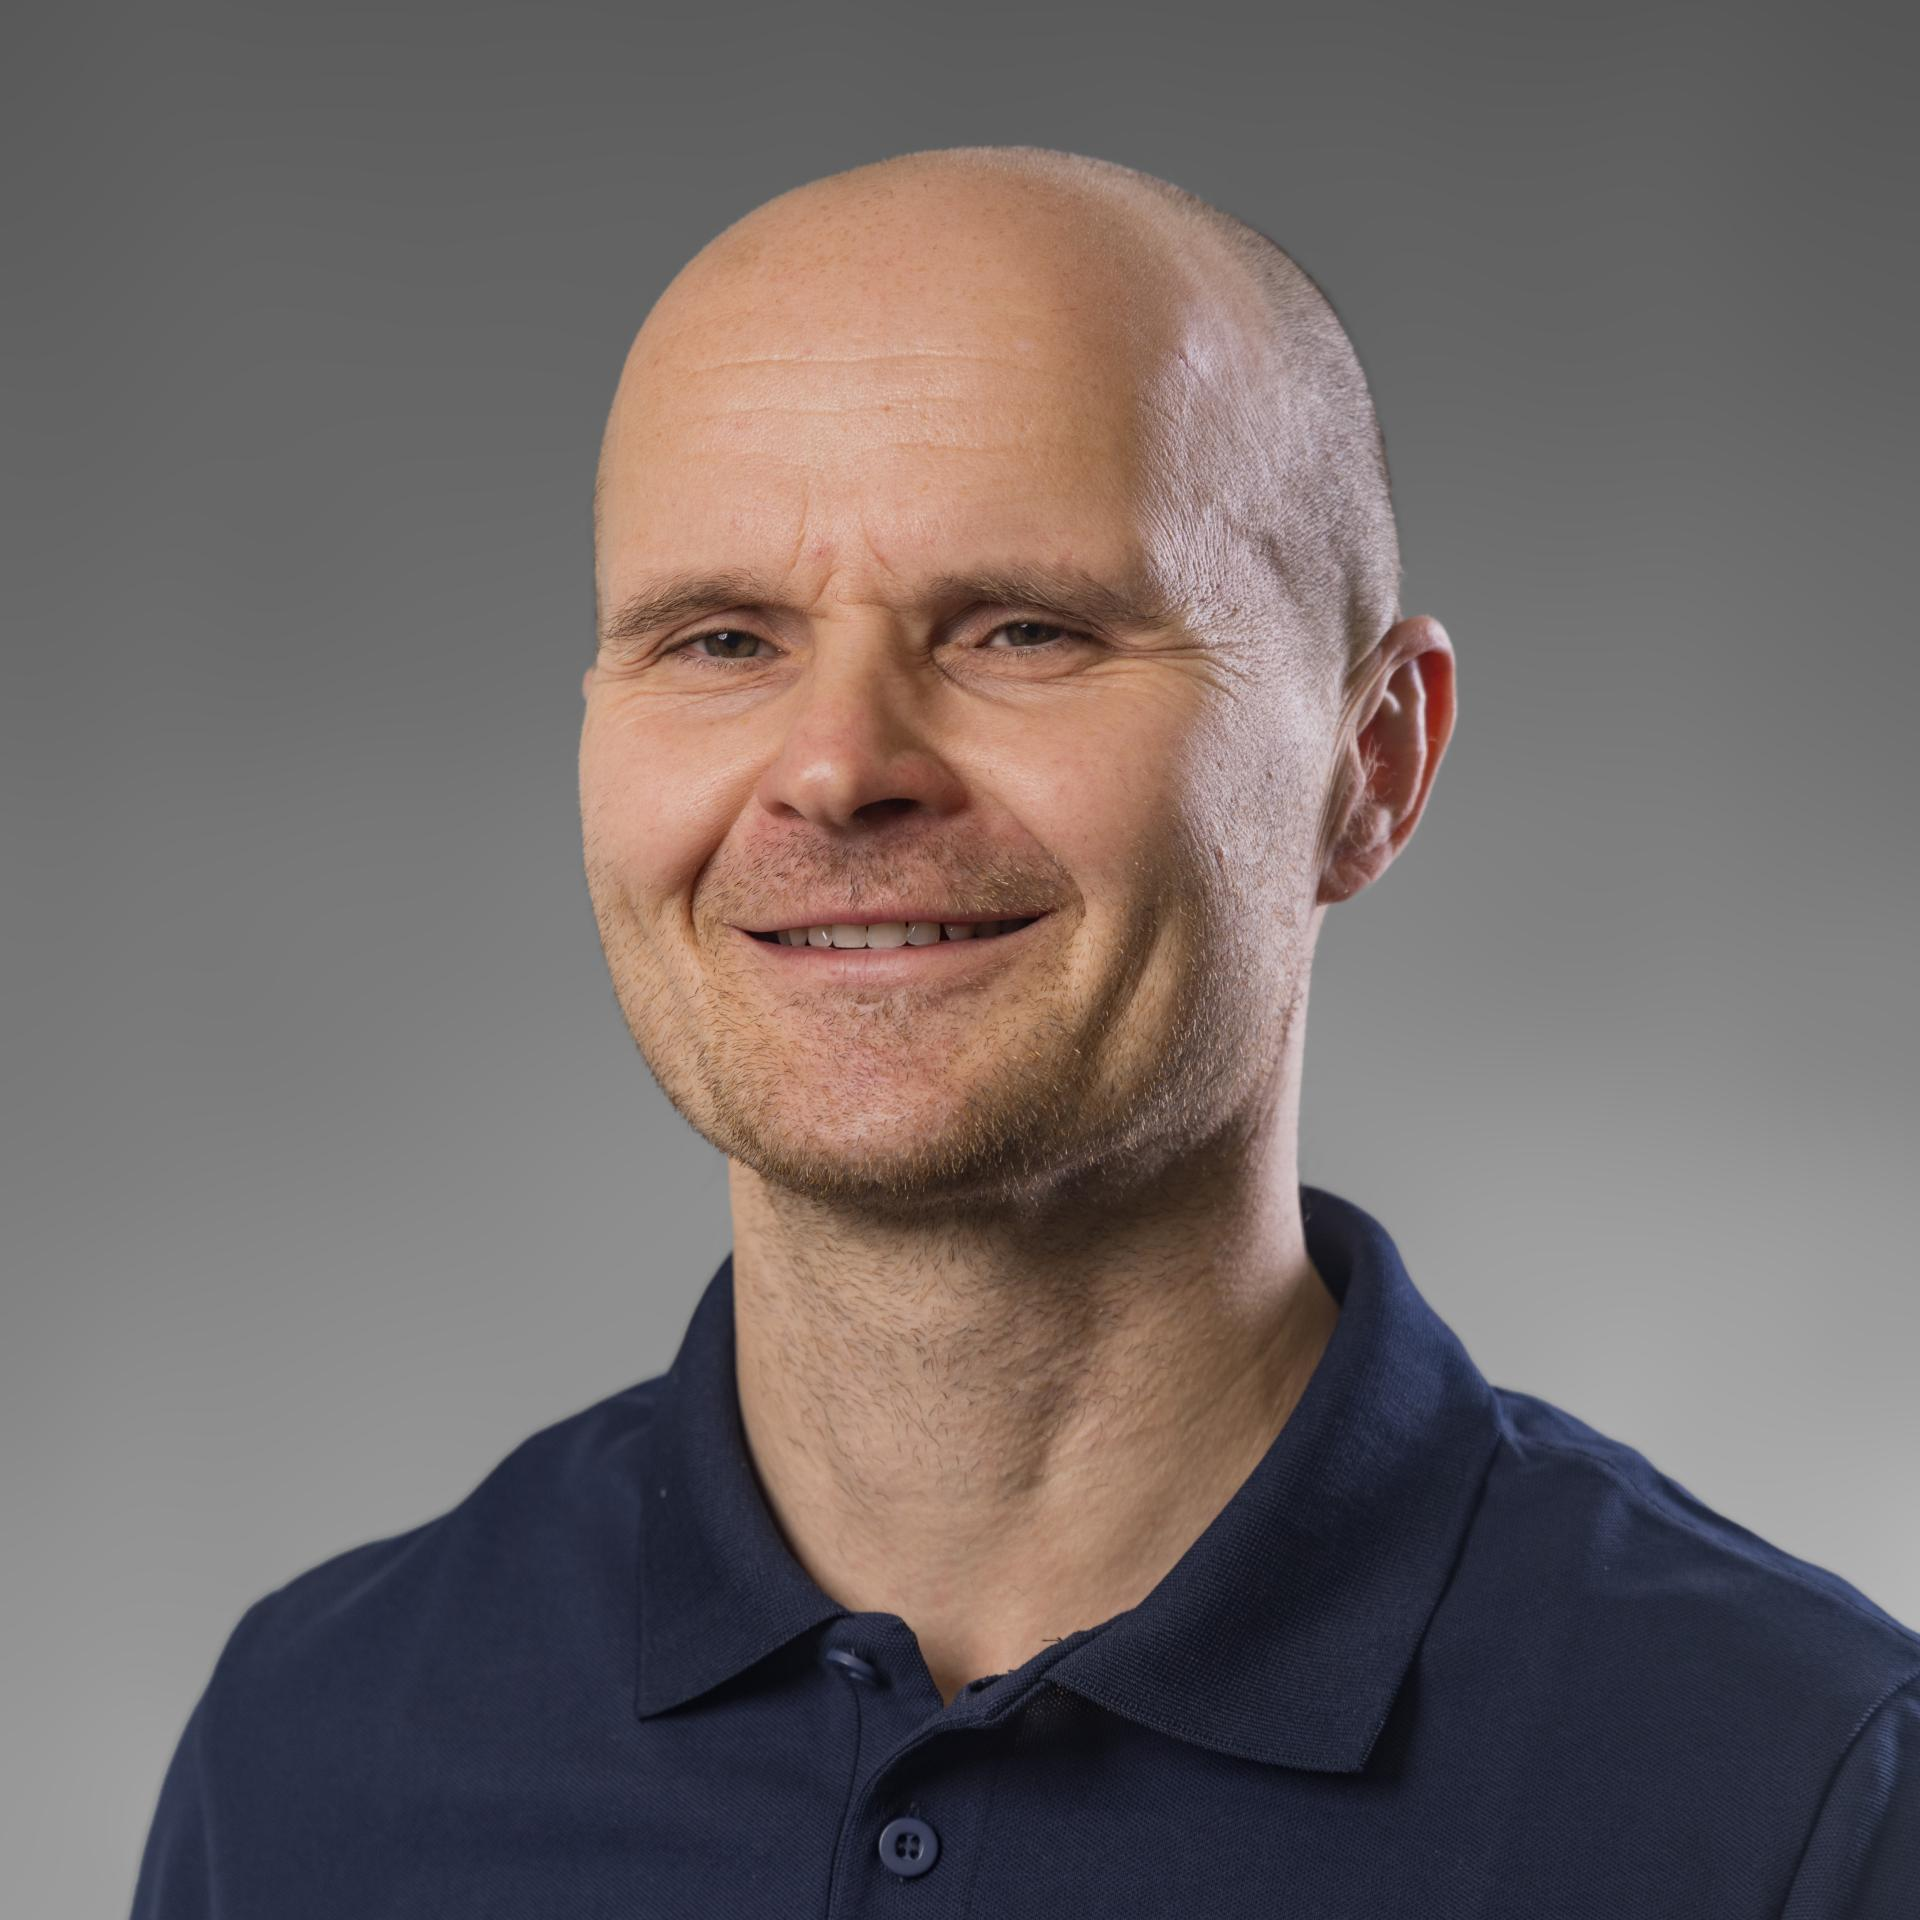
\includegraphics[width=0.8\textwidth]{Antonin-Houska-faceshot.jpg}
      \end{center}
    \end{column}
  \end{columns}
\end{frame}

\begin{frame}
  \frametitle{Álvaro Herrera}

  \begin{columns}
    \begin{column}{0.8\textwidth}
      \begin{itemize}
	\item Álvaro Herrera, \href{mailto:alvherre@kurilemu.de}{alvherre@kurilemu.de}
	\item Postgres contributor since 2002
	\item Working as a Postgres developer for EDB since 2012
      \end{itemize}
    \end{column}
    \begin{column}{0.2\textwidth}
      \begin{center}
	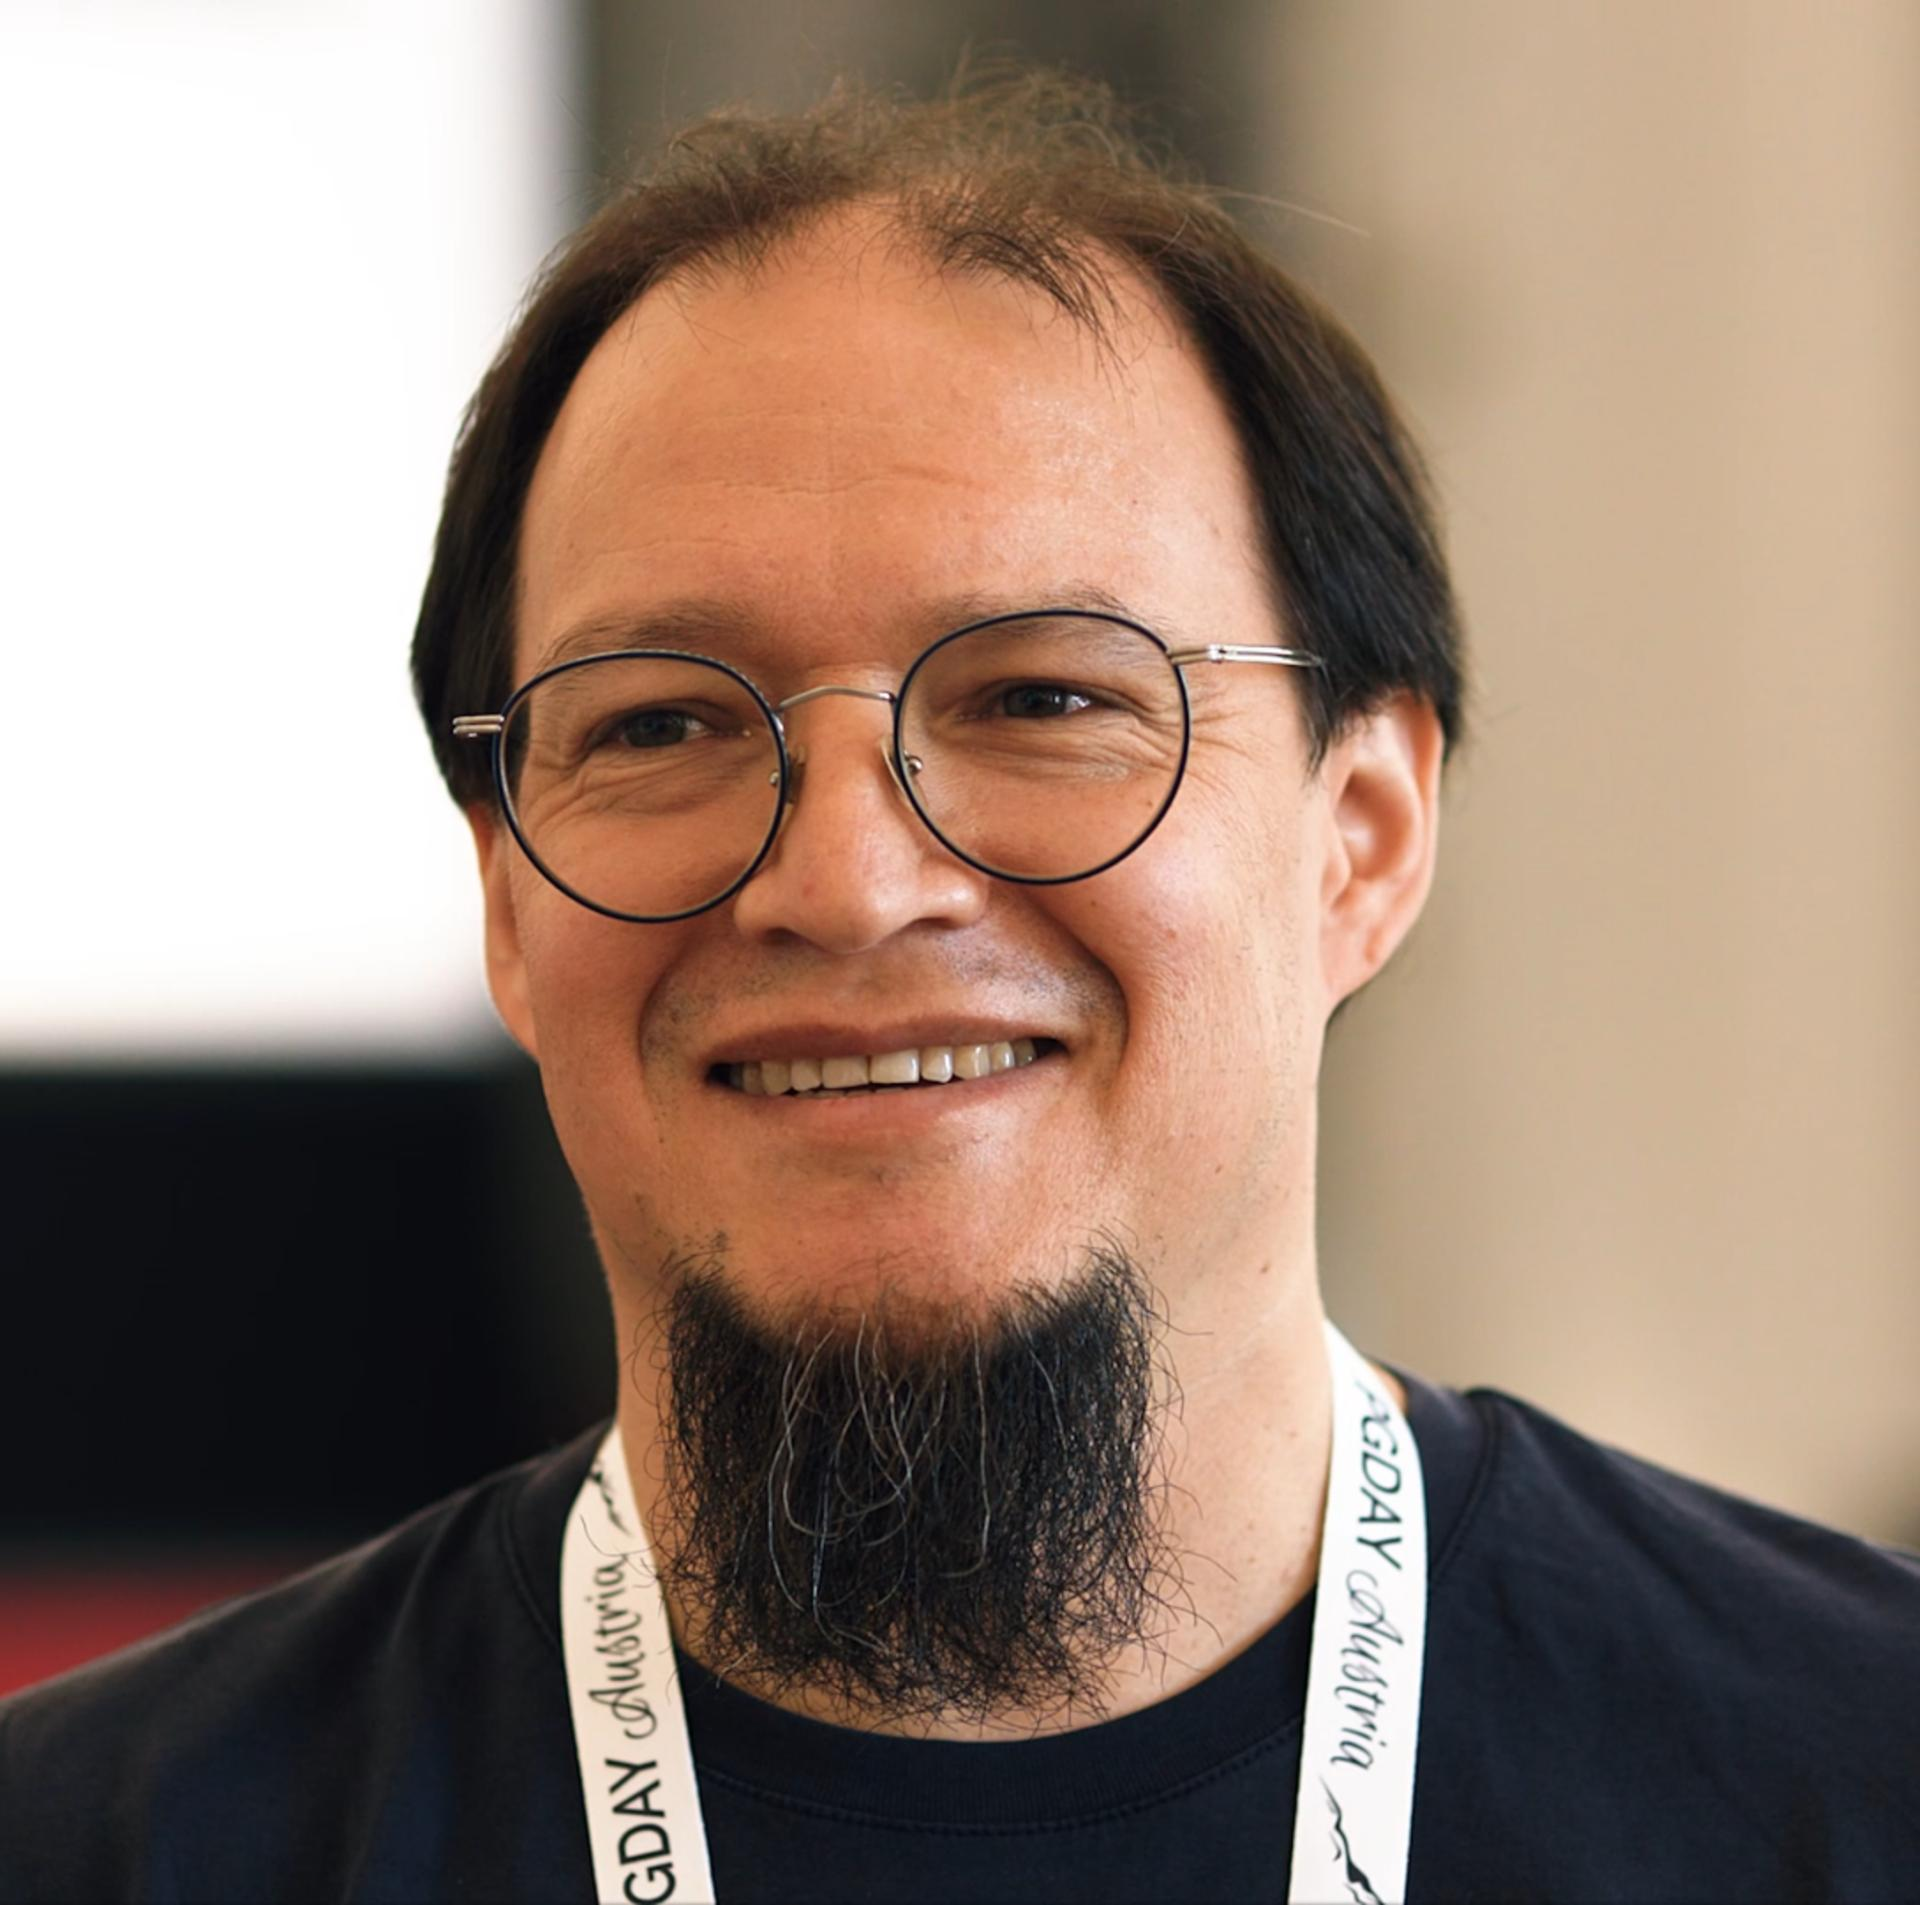
\includegraphics[width=0.8\textwidth]{alvaro-faceshot.jpg}
      \end{center}
    \end{column}
  \end{columns}
\end{frame}

\begin{frame}
  \frametitle{Talk structure}
  \begin{enumerate}
    \item The problem: table bloat
    \item The historical solution: VACUUM and friends
    \item Third-party solutions
      \begin{itemize}
	\item \texttt{pg\_reorg}
	\item \texttt{pg\_repack}
	\item \texttt{pg\_squeeze}
      \end{itemize}
    \item Non-concurrent REPACK
    \item REPACK CONCURRENTLY
  \end{enumerate}
\end{frame}

\section{Historical review}

\begin{frame}
  \frametitle{Table bloat}
  \begin{itemize}
    \item Comes from \emph{non-overwriting} MVCC implementation
    \item Non-overwriting: old versions of updated tuples are not immediately removable
    \item \emph{vacuuming}\footnote{And HOT-pruning.} takes care of them afterwards
  \end{itemize}
\end{frame}

\begin{frame}
  \frametitle{Table bloat: other databases}
  \includegraphics[width=\sizeforimages\textwidth]{images/oracle_01.png}

  An overwriting storage manager might use a ``rollback segment''
\end{frame}

\begin{frame}
  \frametitle{Table bloat: other databases}
  \includegraphics[width=\sizeforimages\textwidth]{images/oracle_02.png}

  As the table is updated, the old versions are moved to the rollback segment. The table doesn't need later cleanup
\end{frame}

\begin{frame}
  \frametitle{A rollback segment?}
  \begin{itemize}
    \item requires handling of disk space for it
    \item and later cleanup
    \item notably: rollbacks are expensive
    \item<2> and is more difficult to implement
    \item<2> Postgres tried: see \texttt{zheap}
    \item<2> Not yet achieved!
  \end{itemize}
\end{frame}

\begin{frame}
  \frametitle{Tuples}
  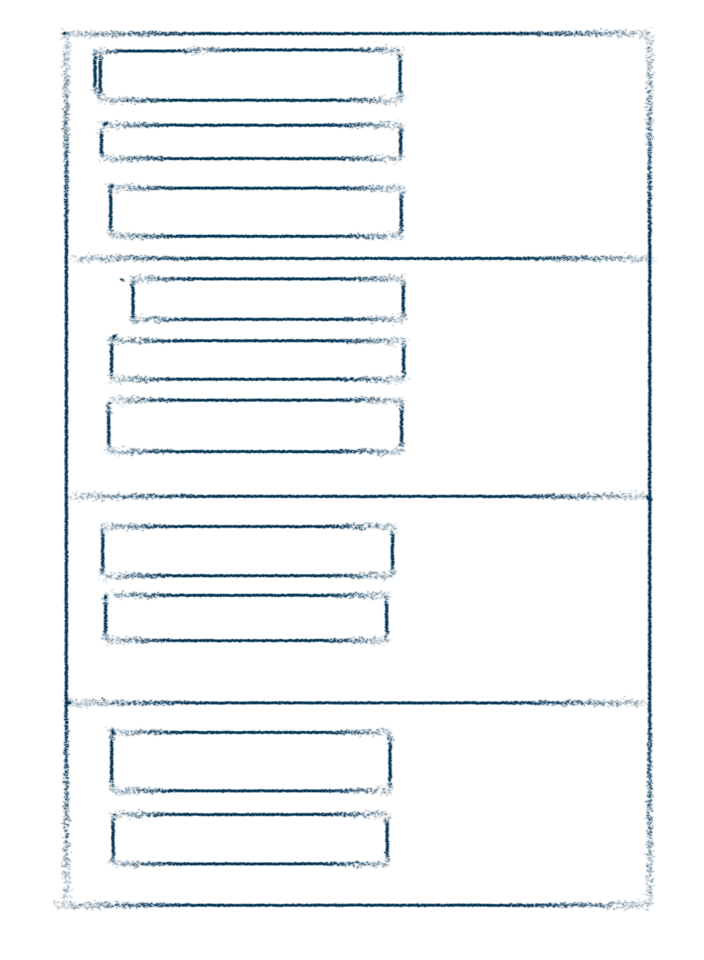
\includegraphics[height=\sizeforimages\textheight]{images/tuples.png}
\end{frame}

\begin{frame}
  \frametitle{Dead tuples}
  \begin{columns}
    \begin{column}{0.5\textwidth}
      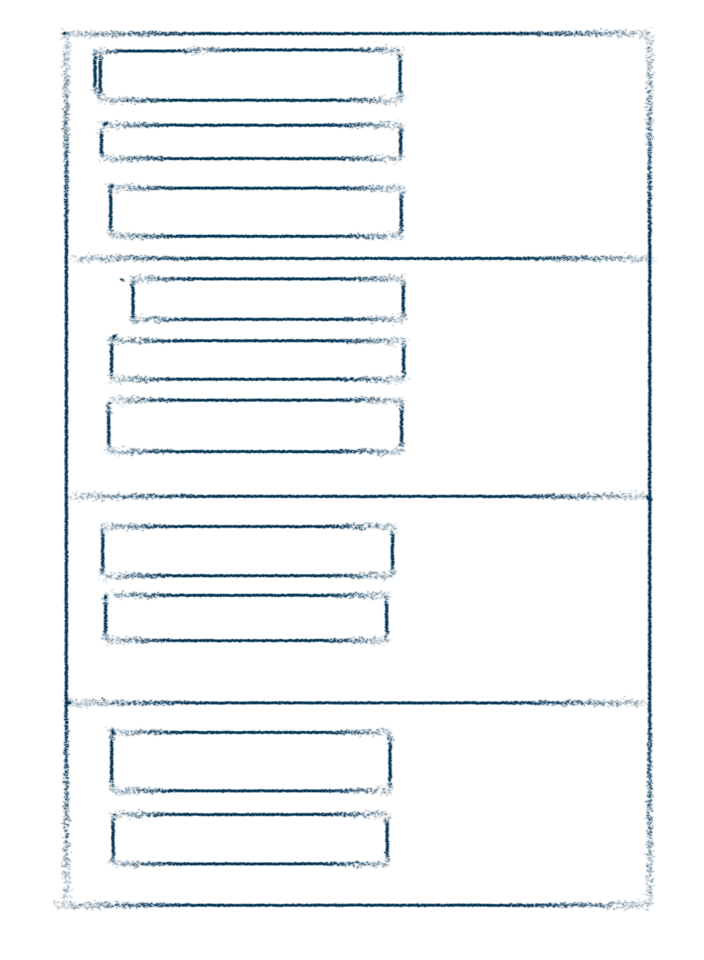
\includegraphics[height=\sizeforimages\textheight]{images/tuples.png}
    \end{column}
    \begin{column}{0.8\textwidth}
      \includegraphics[height=\sizeforimages\textheight]{images/tuples_dead.png}
    \end{column}
  \end{columns}
\end{frame}

\begin{frame}
  \frametitle{VACUUM phase 1: Dead tuples removed}
  \begin{columns}
    \begin{column}{0.5\textwidth}
      \includegraphics[height=\sizeforimages\textheight]{images/tuples_dead.png}
    \end{column}
    \begin{column}{0.8\textwidth}
      \includegraphics[height=\sizeforimages\textheight]{images/tuples_removed.png}
    \end{column}
  \end{columns}
\end{frame}

\begin{frame}
  \frametitle{VACUUM phase 2: Compact table}
  \begin{columns}
    \begin{column}{0.5\textwidth}
      \includegraphics[height=\sizeforimages\textheight]{images/tuples_removed.png}

    \end{column}
    \begin{column}{0.8\textwidth}
      \includegraphics[height=\sizeforimages\textheight]{images/tuples_moving.png}
    \end{column}
  \end{columns}
\end{frame}

\begin{frame}
  \frametitle{``Lazy'' vacuum}
  \begin{itemize}
    \item But this required ``access exclusive'' lock on the table
    \item In 2001 (Postgres 7.2), Tom Lane introduces ``lazy vacuum''
      % commit 4046e58c2478cfcdd4334e2c282b5a42f047ea0b
    \item Doesn't require access exclusive lock anymore
    \item Operation can continue
    \item Disadvantage: surviving tuples cannot be moved across pages
    \item Old-style vacuum is renamed \texttt{VACUUM FULL}
  \end{itemize}
\end{frame}



\begin{frame}
  \frametitle{The problem: table bloat}
  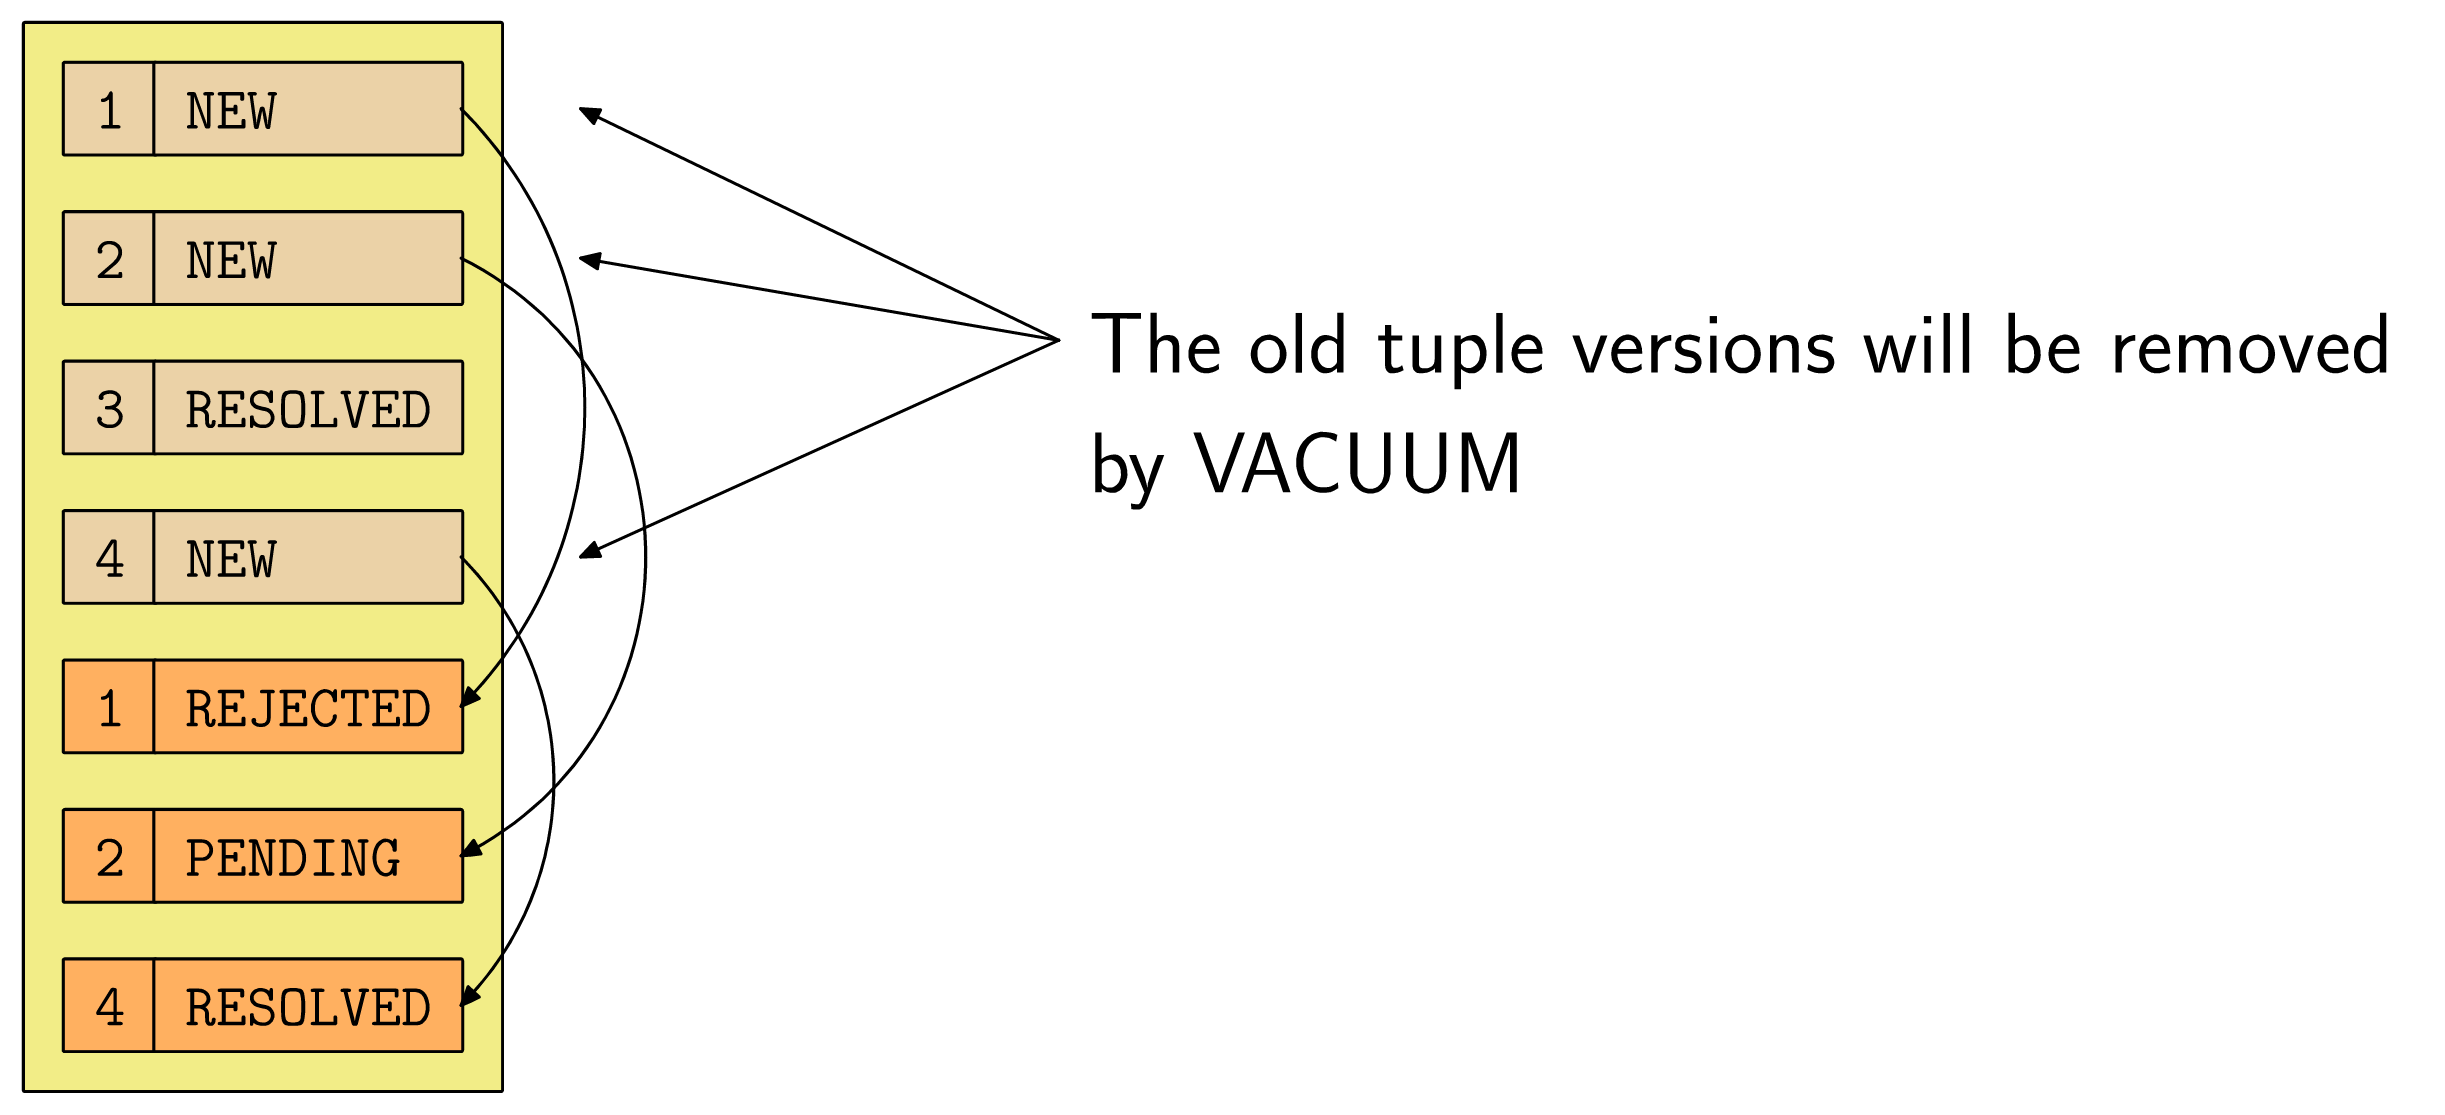
\includegraphics[height=\sizeforimages\textheight]{images/bloat_01.png}
\end{frame}

\begin{frame}
  \frametitle{The problem: table bloat}
  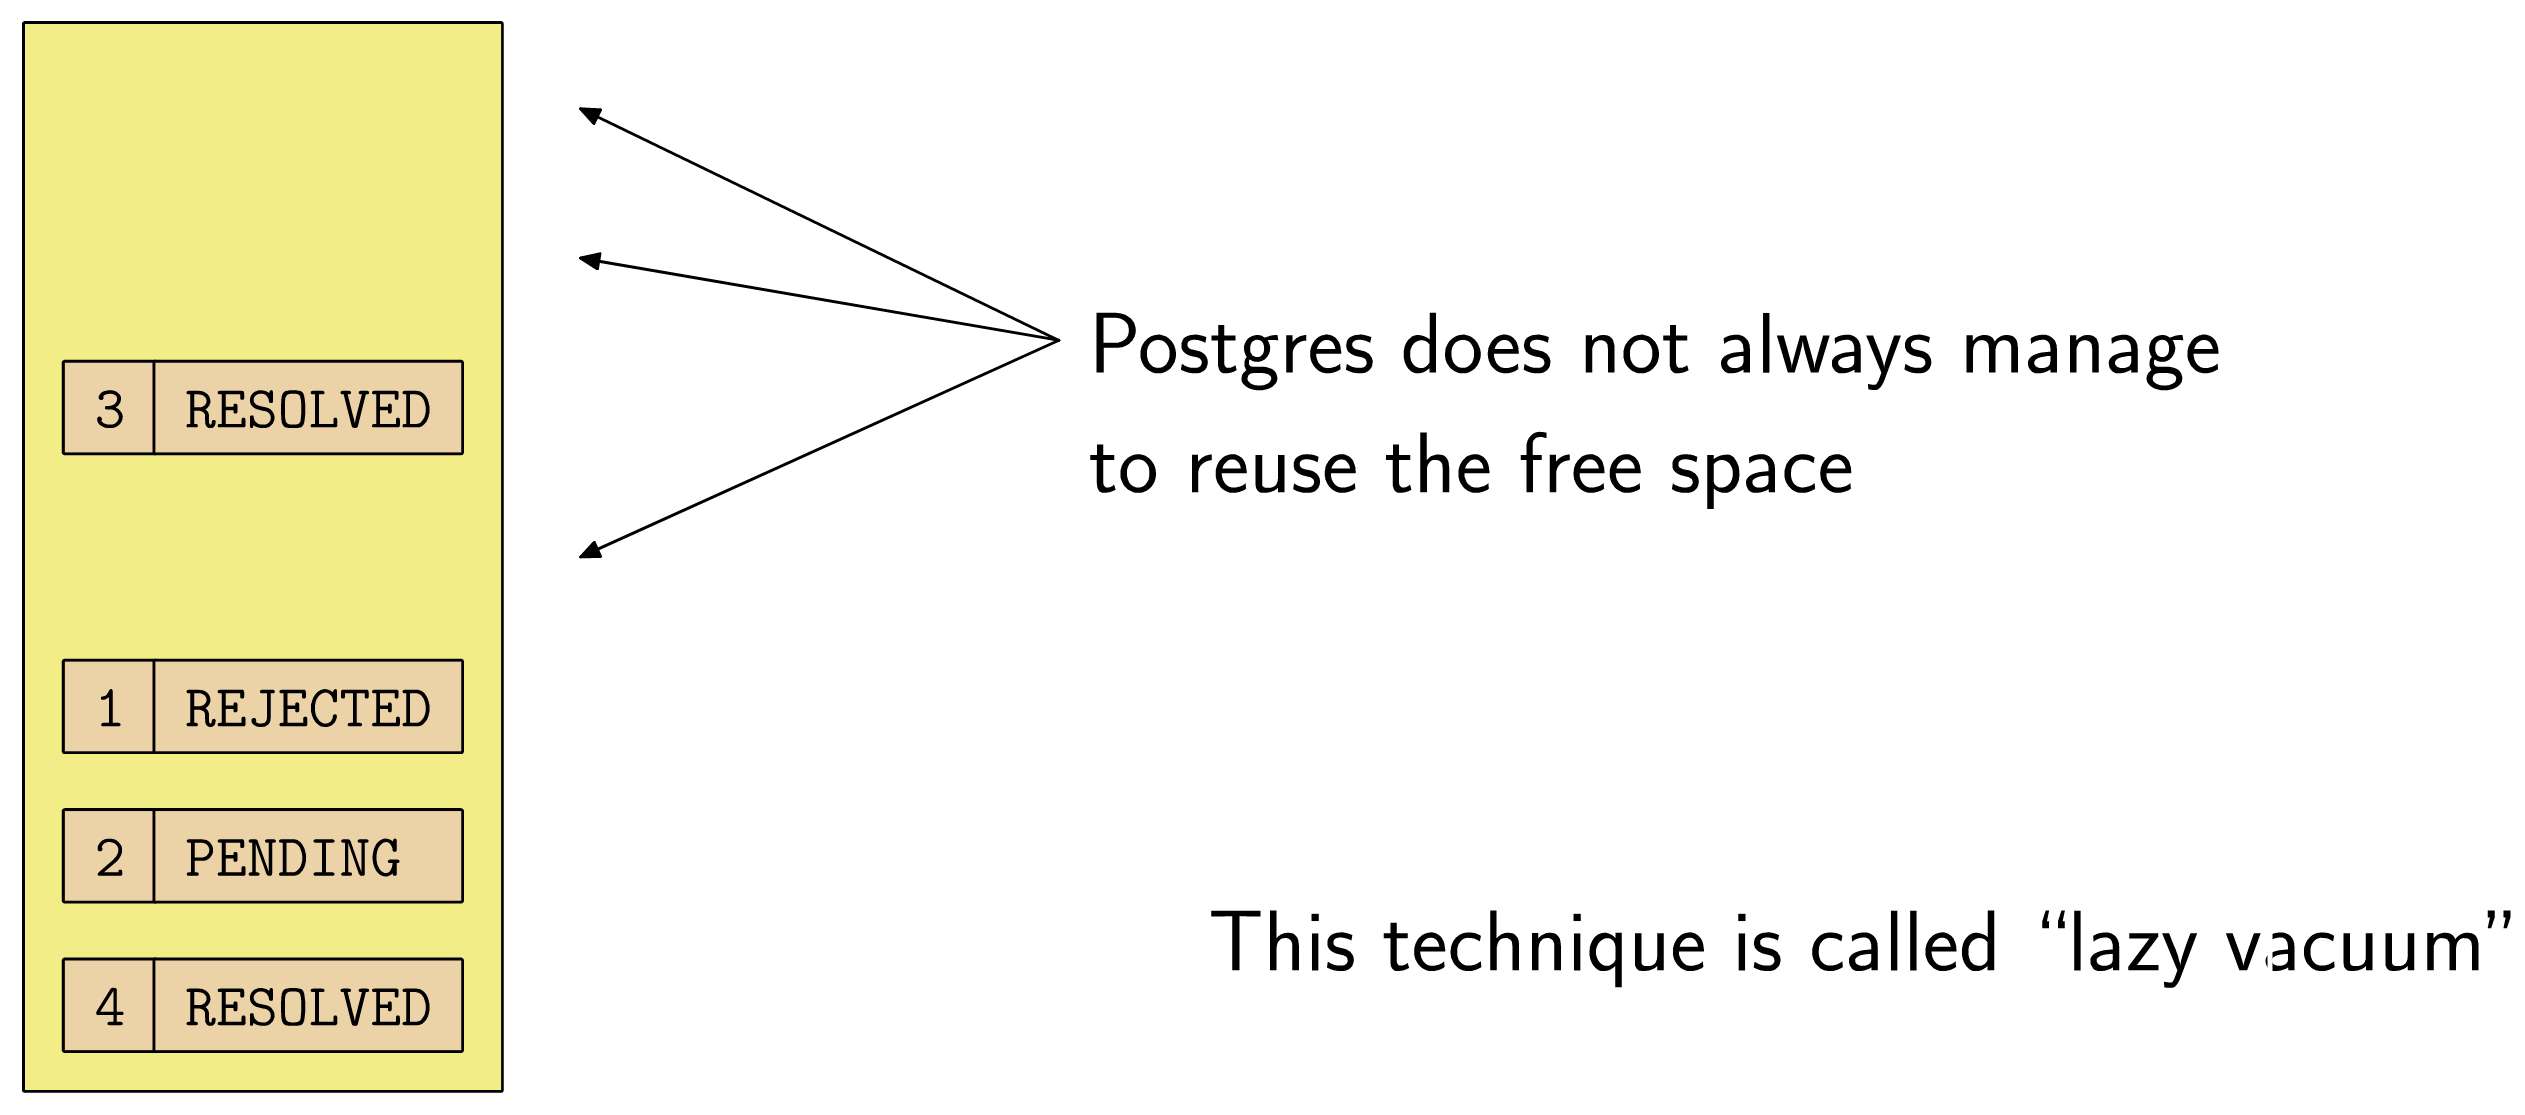
\includegraphics[height=\sizeforimages\textheight]{images/bloat_02.png}
\end{frame}

\begin{frame}
  \frametitle{Faster VACUUM FULL}
  \begin{itemize}
    \item In 2010 (Postgres 9.0), VACUUM FULL was changed to use the CLUSTER code
      % commit 946cf229e89fda779161d707f3ba1f4d3cd024a1
    \item This code creates new storage and copies all live tuples there
    \item Then the new storage is removed
    \item Still requires \emph{access exclusive} lock!
    \item ... but it's much faster
  \end{itemize}
\end{frame}

\begin{frame}
  \frametitle{VACUUM FULL}
  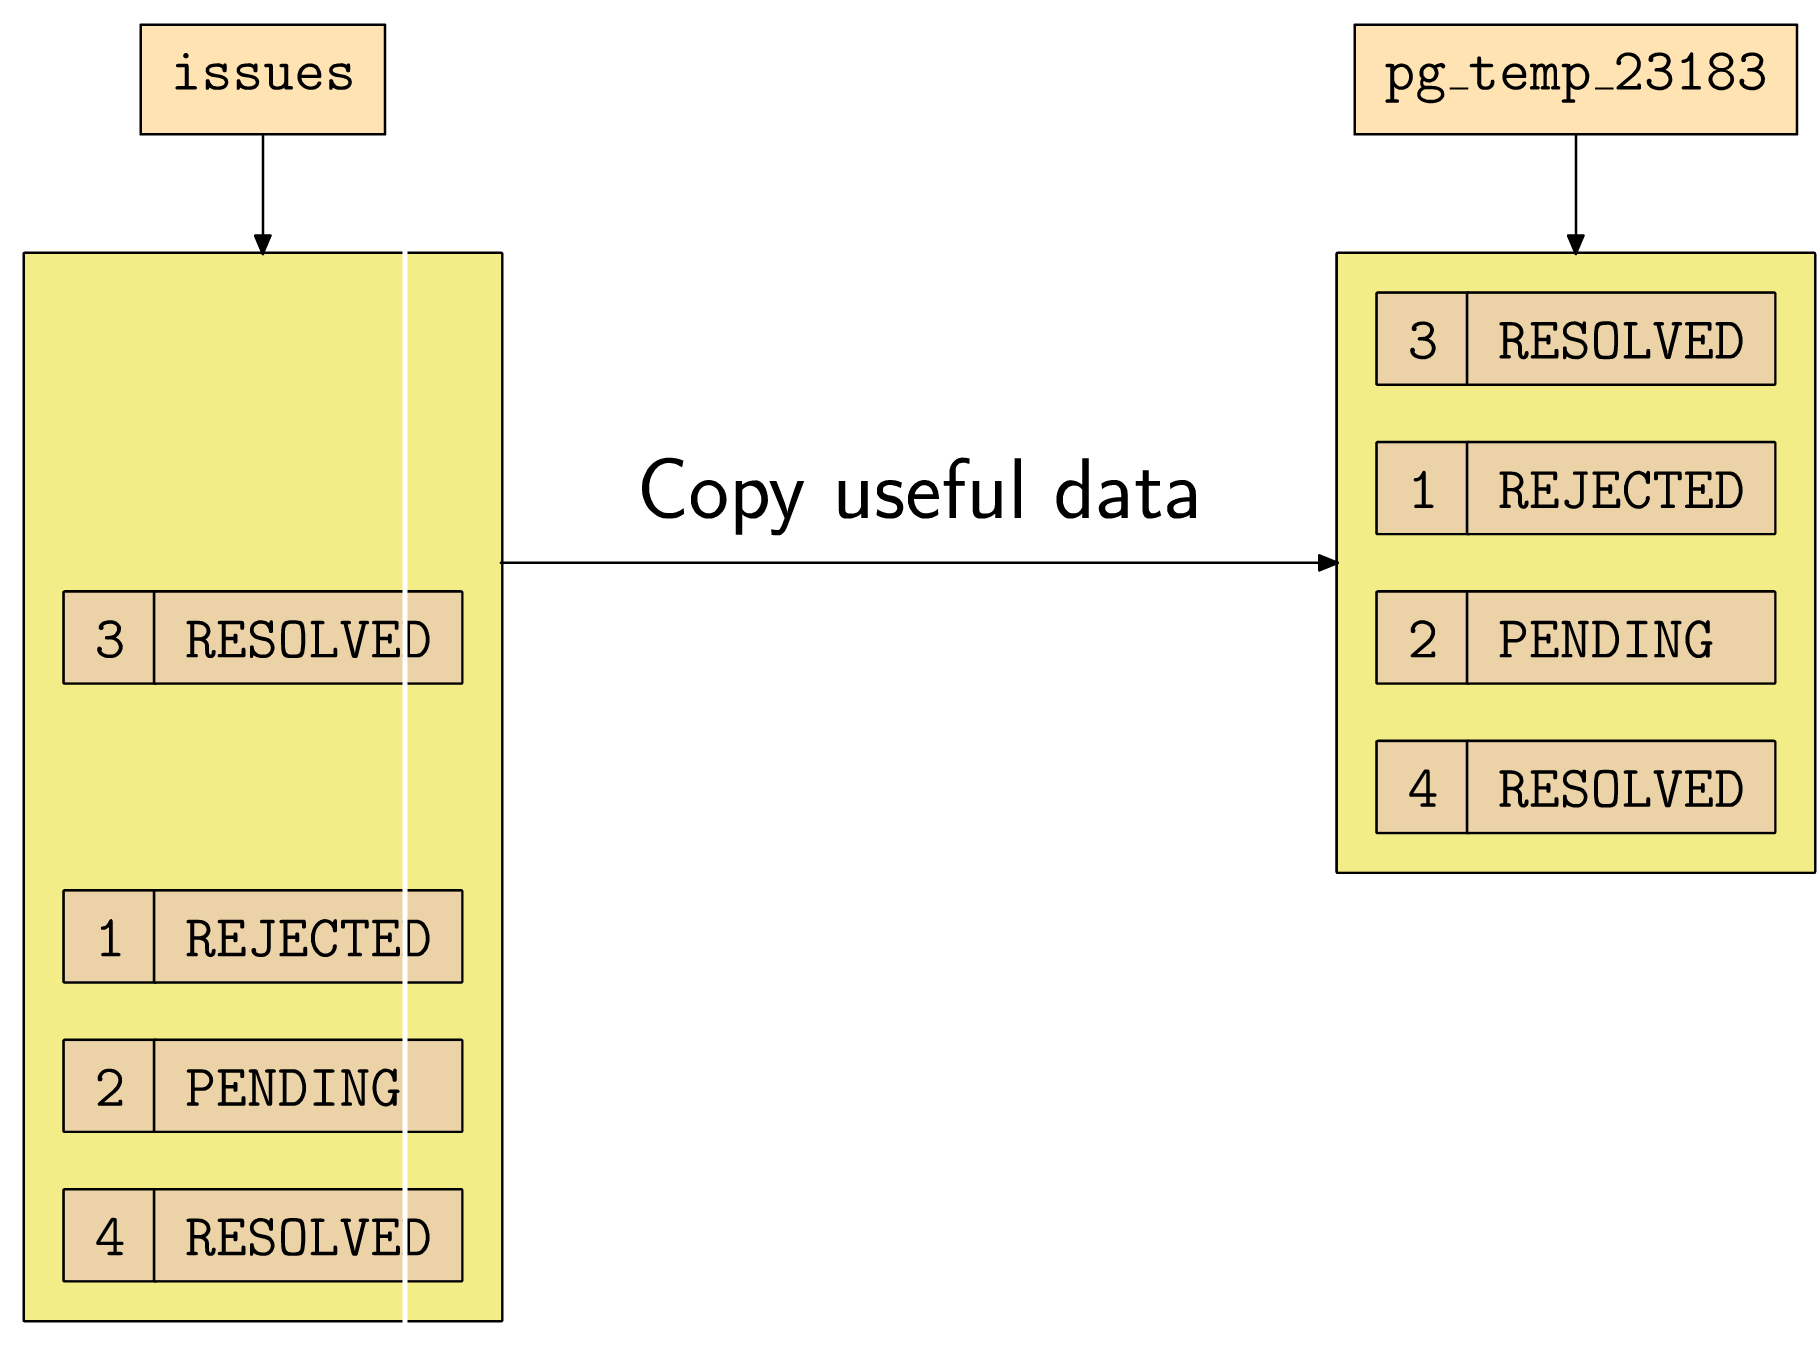
\includegraphics[height=\sizeforimages\textheight]{images/vacuum_full_01.png}
\end{frame}

\begin{frame}
  \frametitle{VACUUM FULL}
  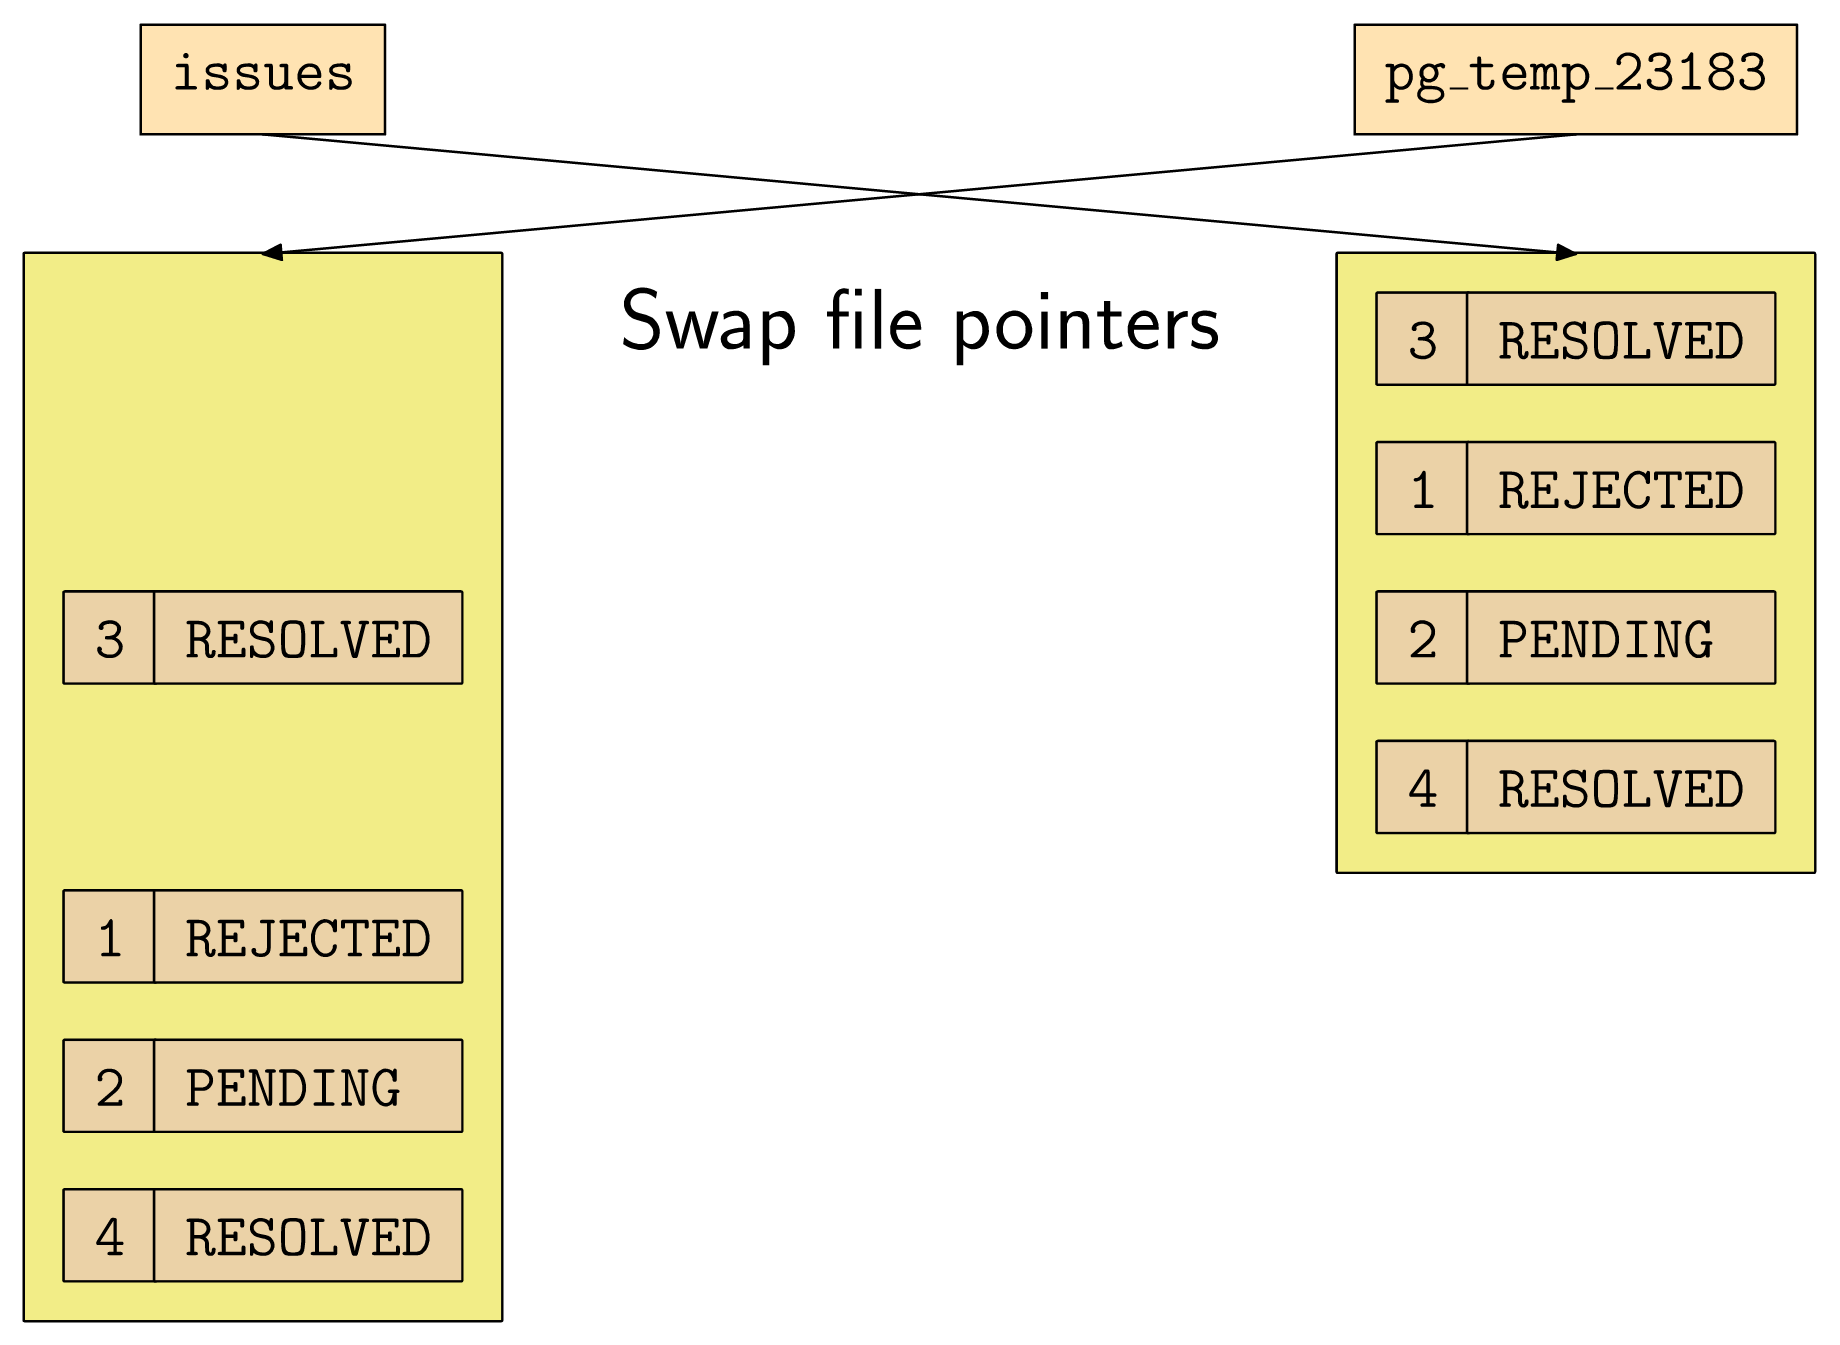
\includegraphics[height=\sizeforimages\textheight]{images/vacuum_full_02.png}
\end{frame}

\begin{frame}
  \frametitle{Exclusive lock is needed}
  \begin{center}
    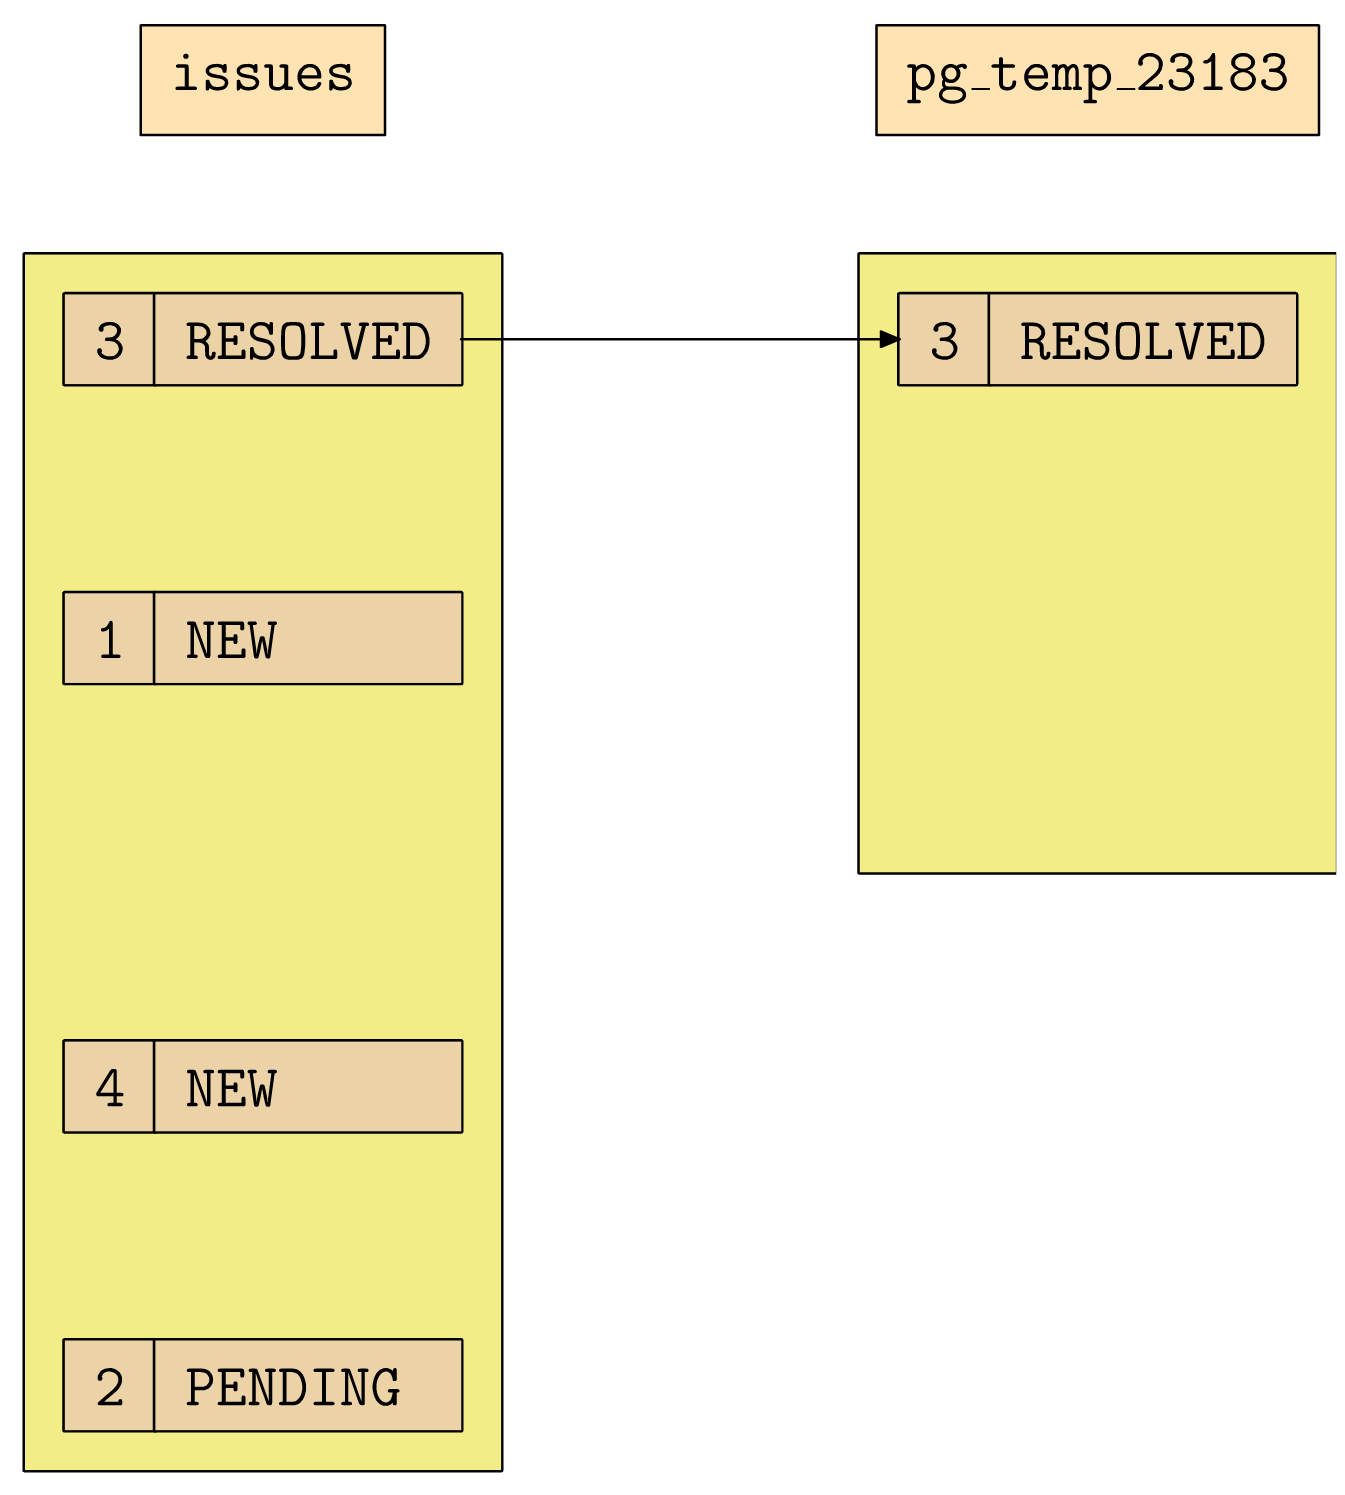
\includegraphics[height=\sizeforimages\textheight]{images/exclusive_lock_needed_01.png}
  \end{center}
\end{frame}

\begin{frame}
  \frametitle{Exclusive lock is needed}
  \begin{center}
    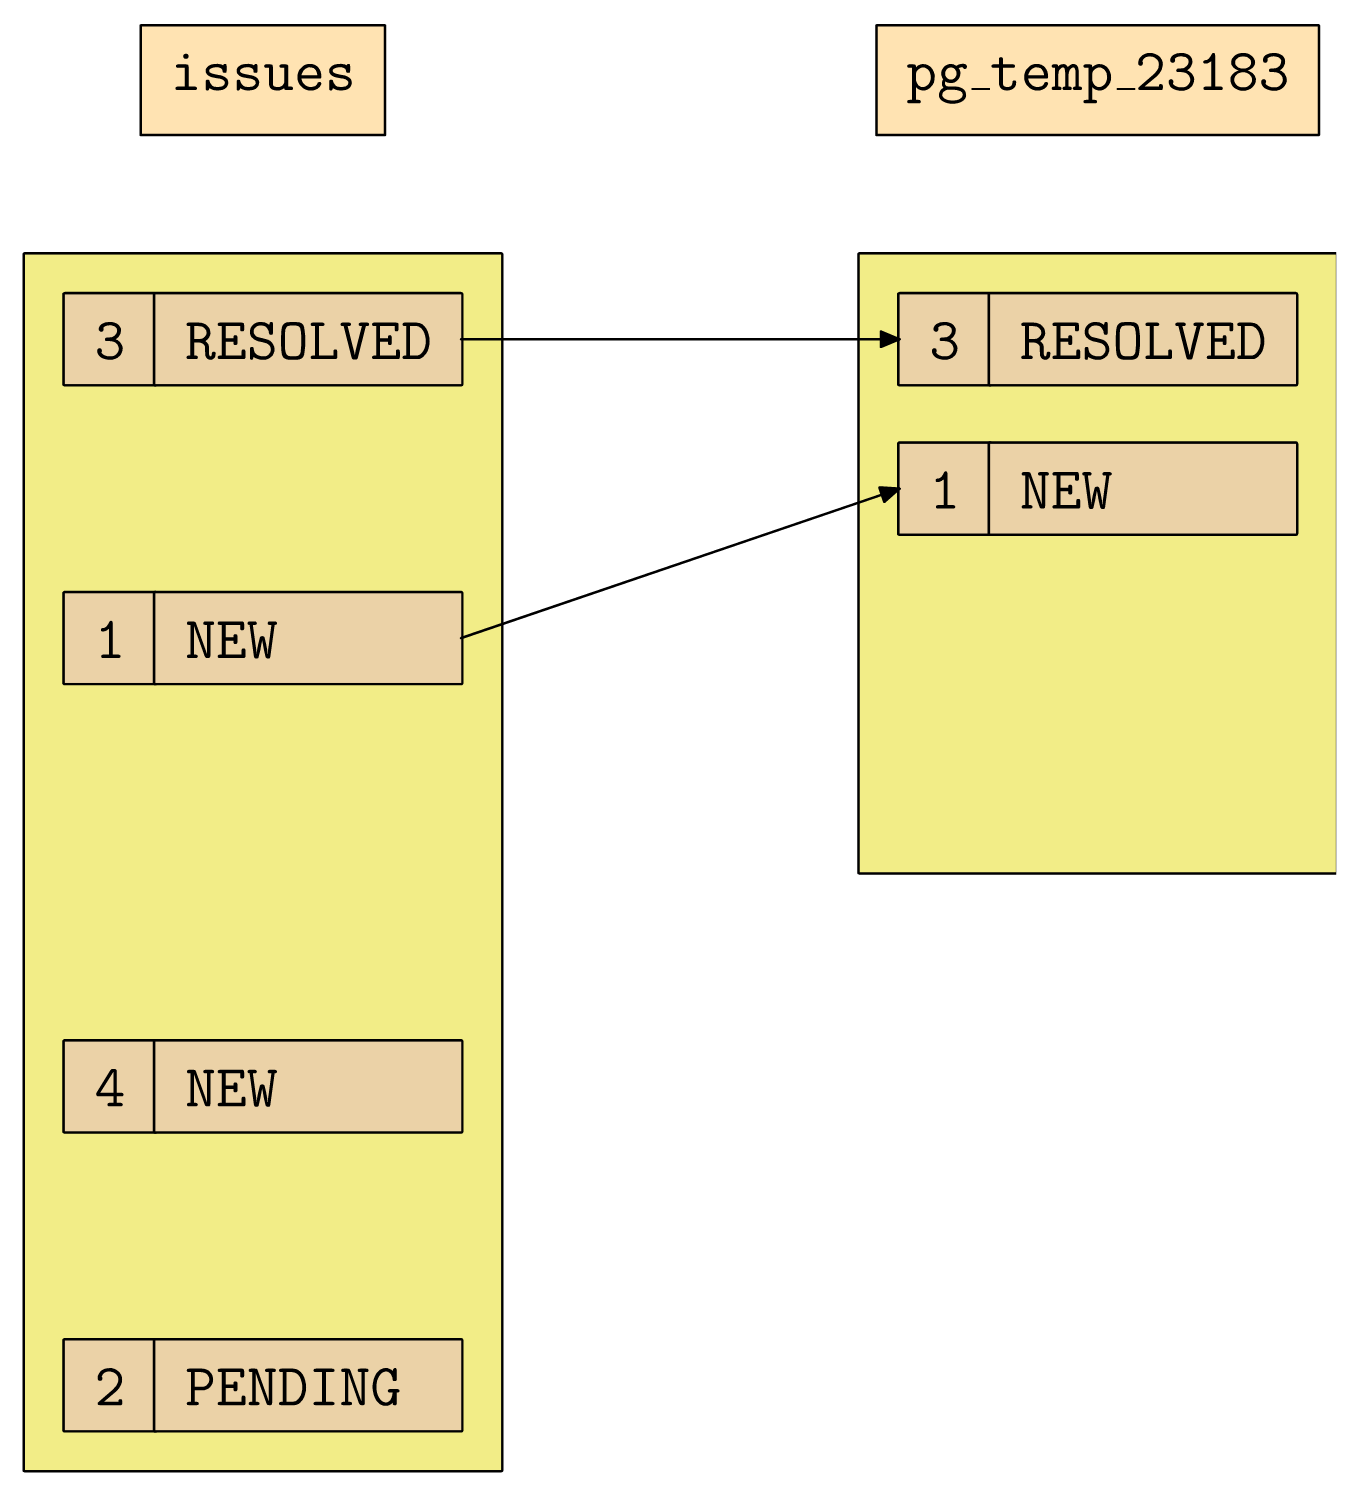
\includegraphics[height=\sizeforimages\textheight]{images/exclusive_lock_needed_02.png}
  \end{center}
\end{frame}

\begin{frame}
  \frametitle{Exclusive lock is needed}
  \begin{center}
    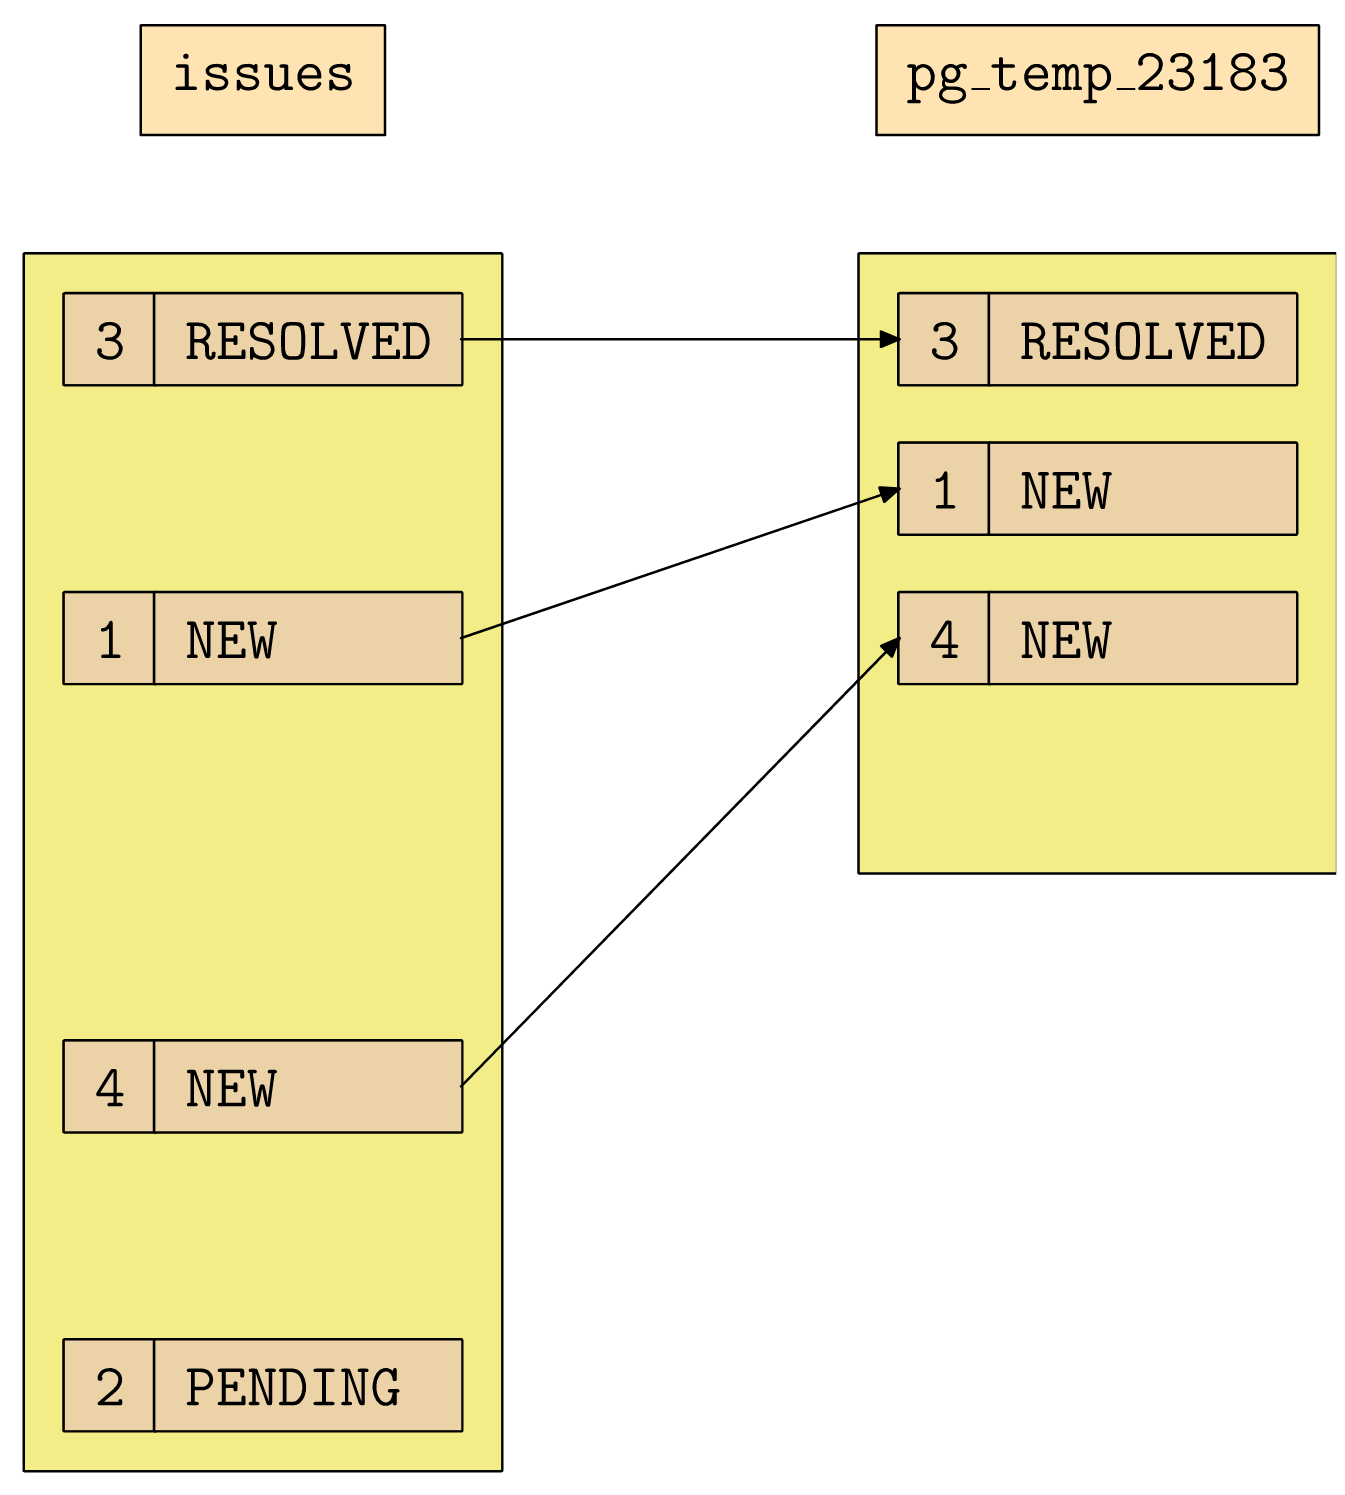
\includegraphics[height=\sizeforimages\textheight]{images/exclusive_lock_needed_03.png}
  \end{center}
\end{frame}

\begin{frame}
  \frametitle{Exclusive lock is needed}
  \begin{center}
    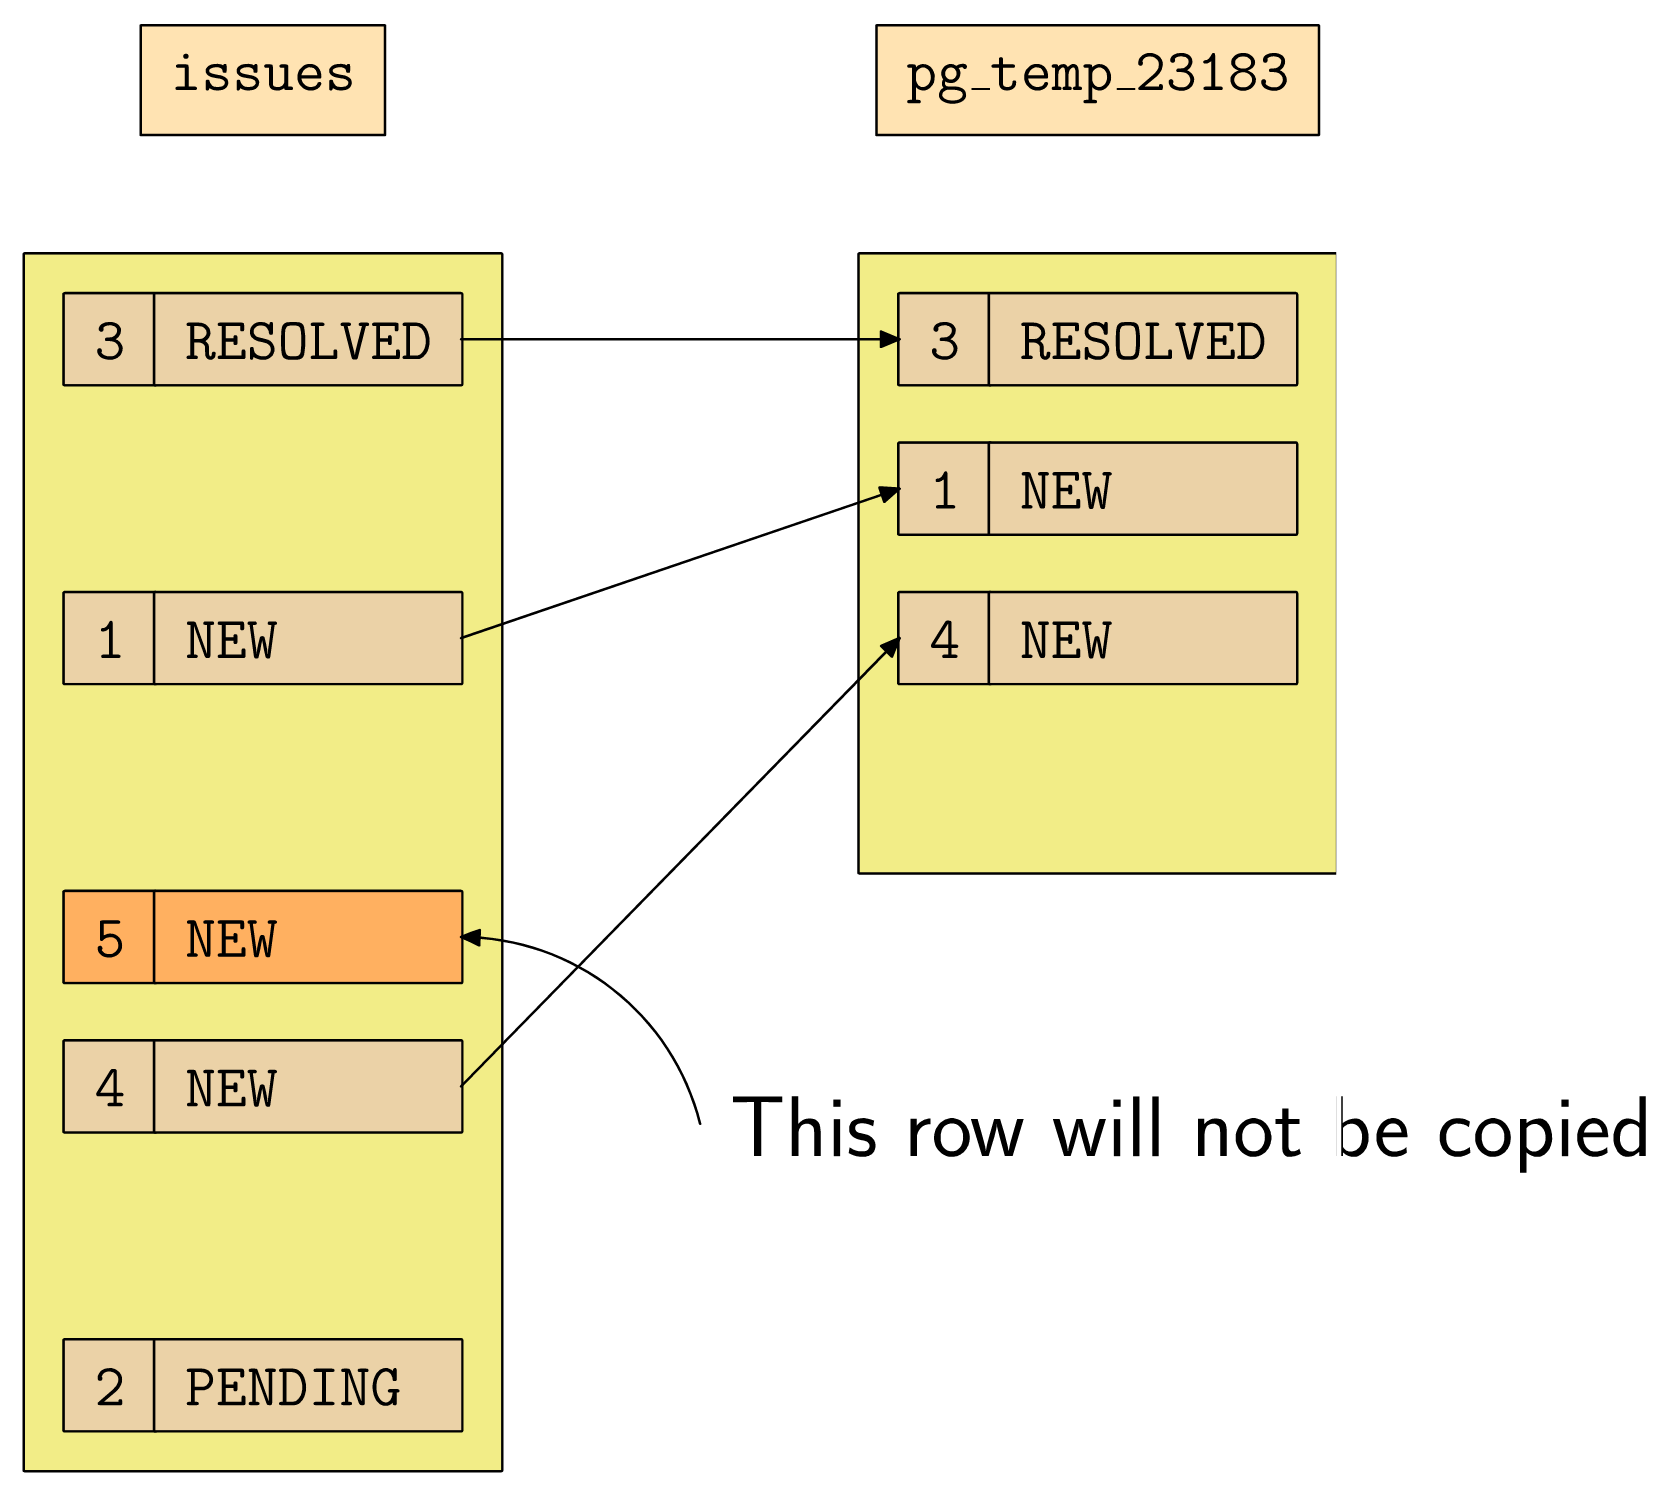
\includegraphics[height=\sizeforimages\textheight]{images/exclusive_lock_needed_04.png}
  \end{center}
\end{frame}

\begin{frame}
  \frametitle{\texttt{pg\_reorg}}
  \begin{itemize}
    \item Created in 2008 by NTT
    \item \href{https://ossc-db.github.io/pg_reorg/pg_reorg.html}{\texttt{https://ossc-db.github.io/pg\_reorg/}}
      \begin{quote}
	``The module is developed to be a better alternative of CLUSTER and VACUUM FULL.''
      \end{quote}
    \item Featured in Depesz's blog in 2011: \href{https://www.depesz.com/2011/07/06/bloat-happens/}{Bloat Happens}
      \begin{quote}
	``All in all – it's a great tool, which does amazing job.''
      \end{quote}
    \item Last release was 1.1.9 in 2013
    \item Pronounced dead in 2020
  \end{itemize}
\end{frame}

\begin{frame}
  \frametitle{\texttt{pg\_repack}}
  \begin{itemize}
    \item Forked from \texttt{pg\_reorg} in 2012
    \item Implemented in two parts:
      \begin{itemize}
	\item A few server-side SQL and C functions
	\item Workflow controlled by a client application
      \end{itemize}
  \end{itemize}
\end{frame}

\begin{frame}
  \frametitle{\texttt{pg\_repack}}
  \begin{center}
    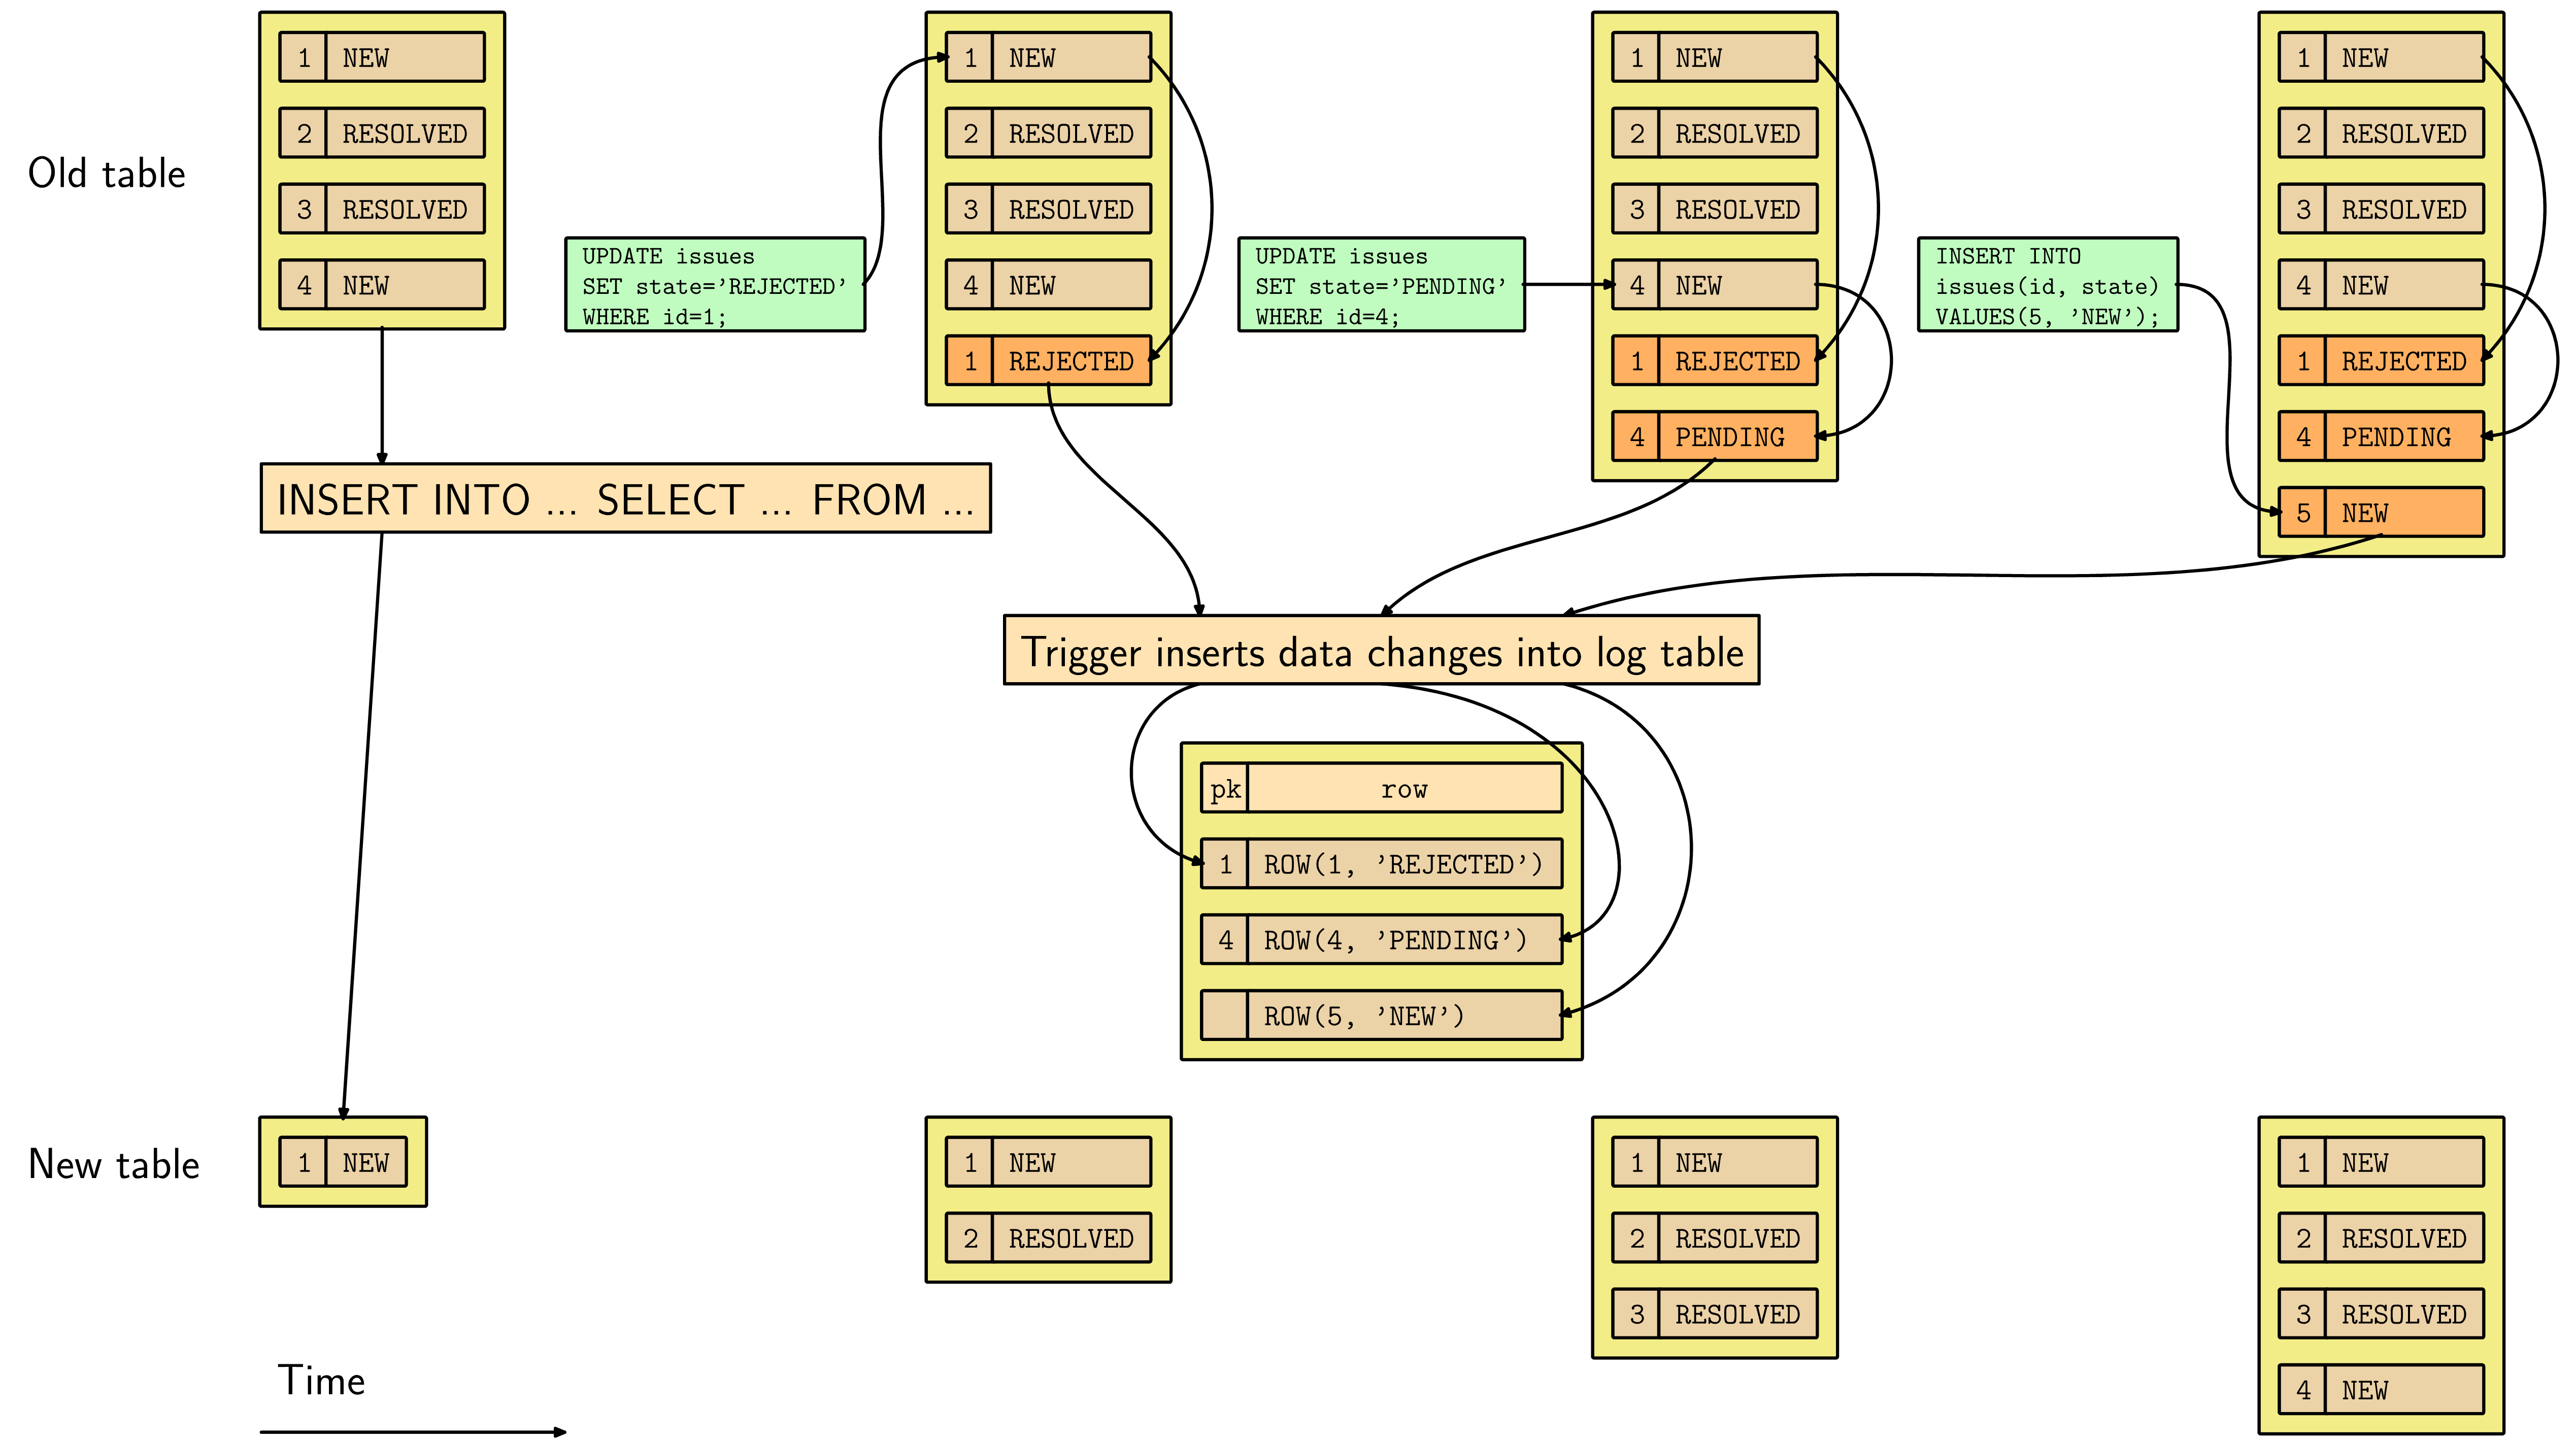
\includegraphics[height=\sizeforimages\textheight]{images/pg_repack_01.png}
  \end{center}
\end{frame}

\begin{frame}
  \frametitle{\texttt{pg\_repack}}
  \begin{center}
    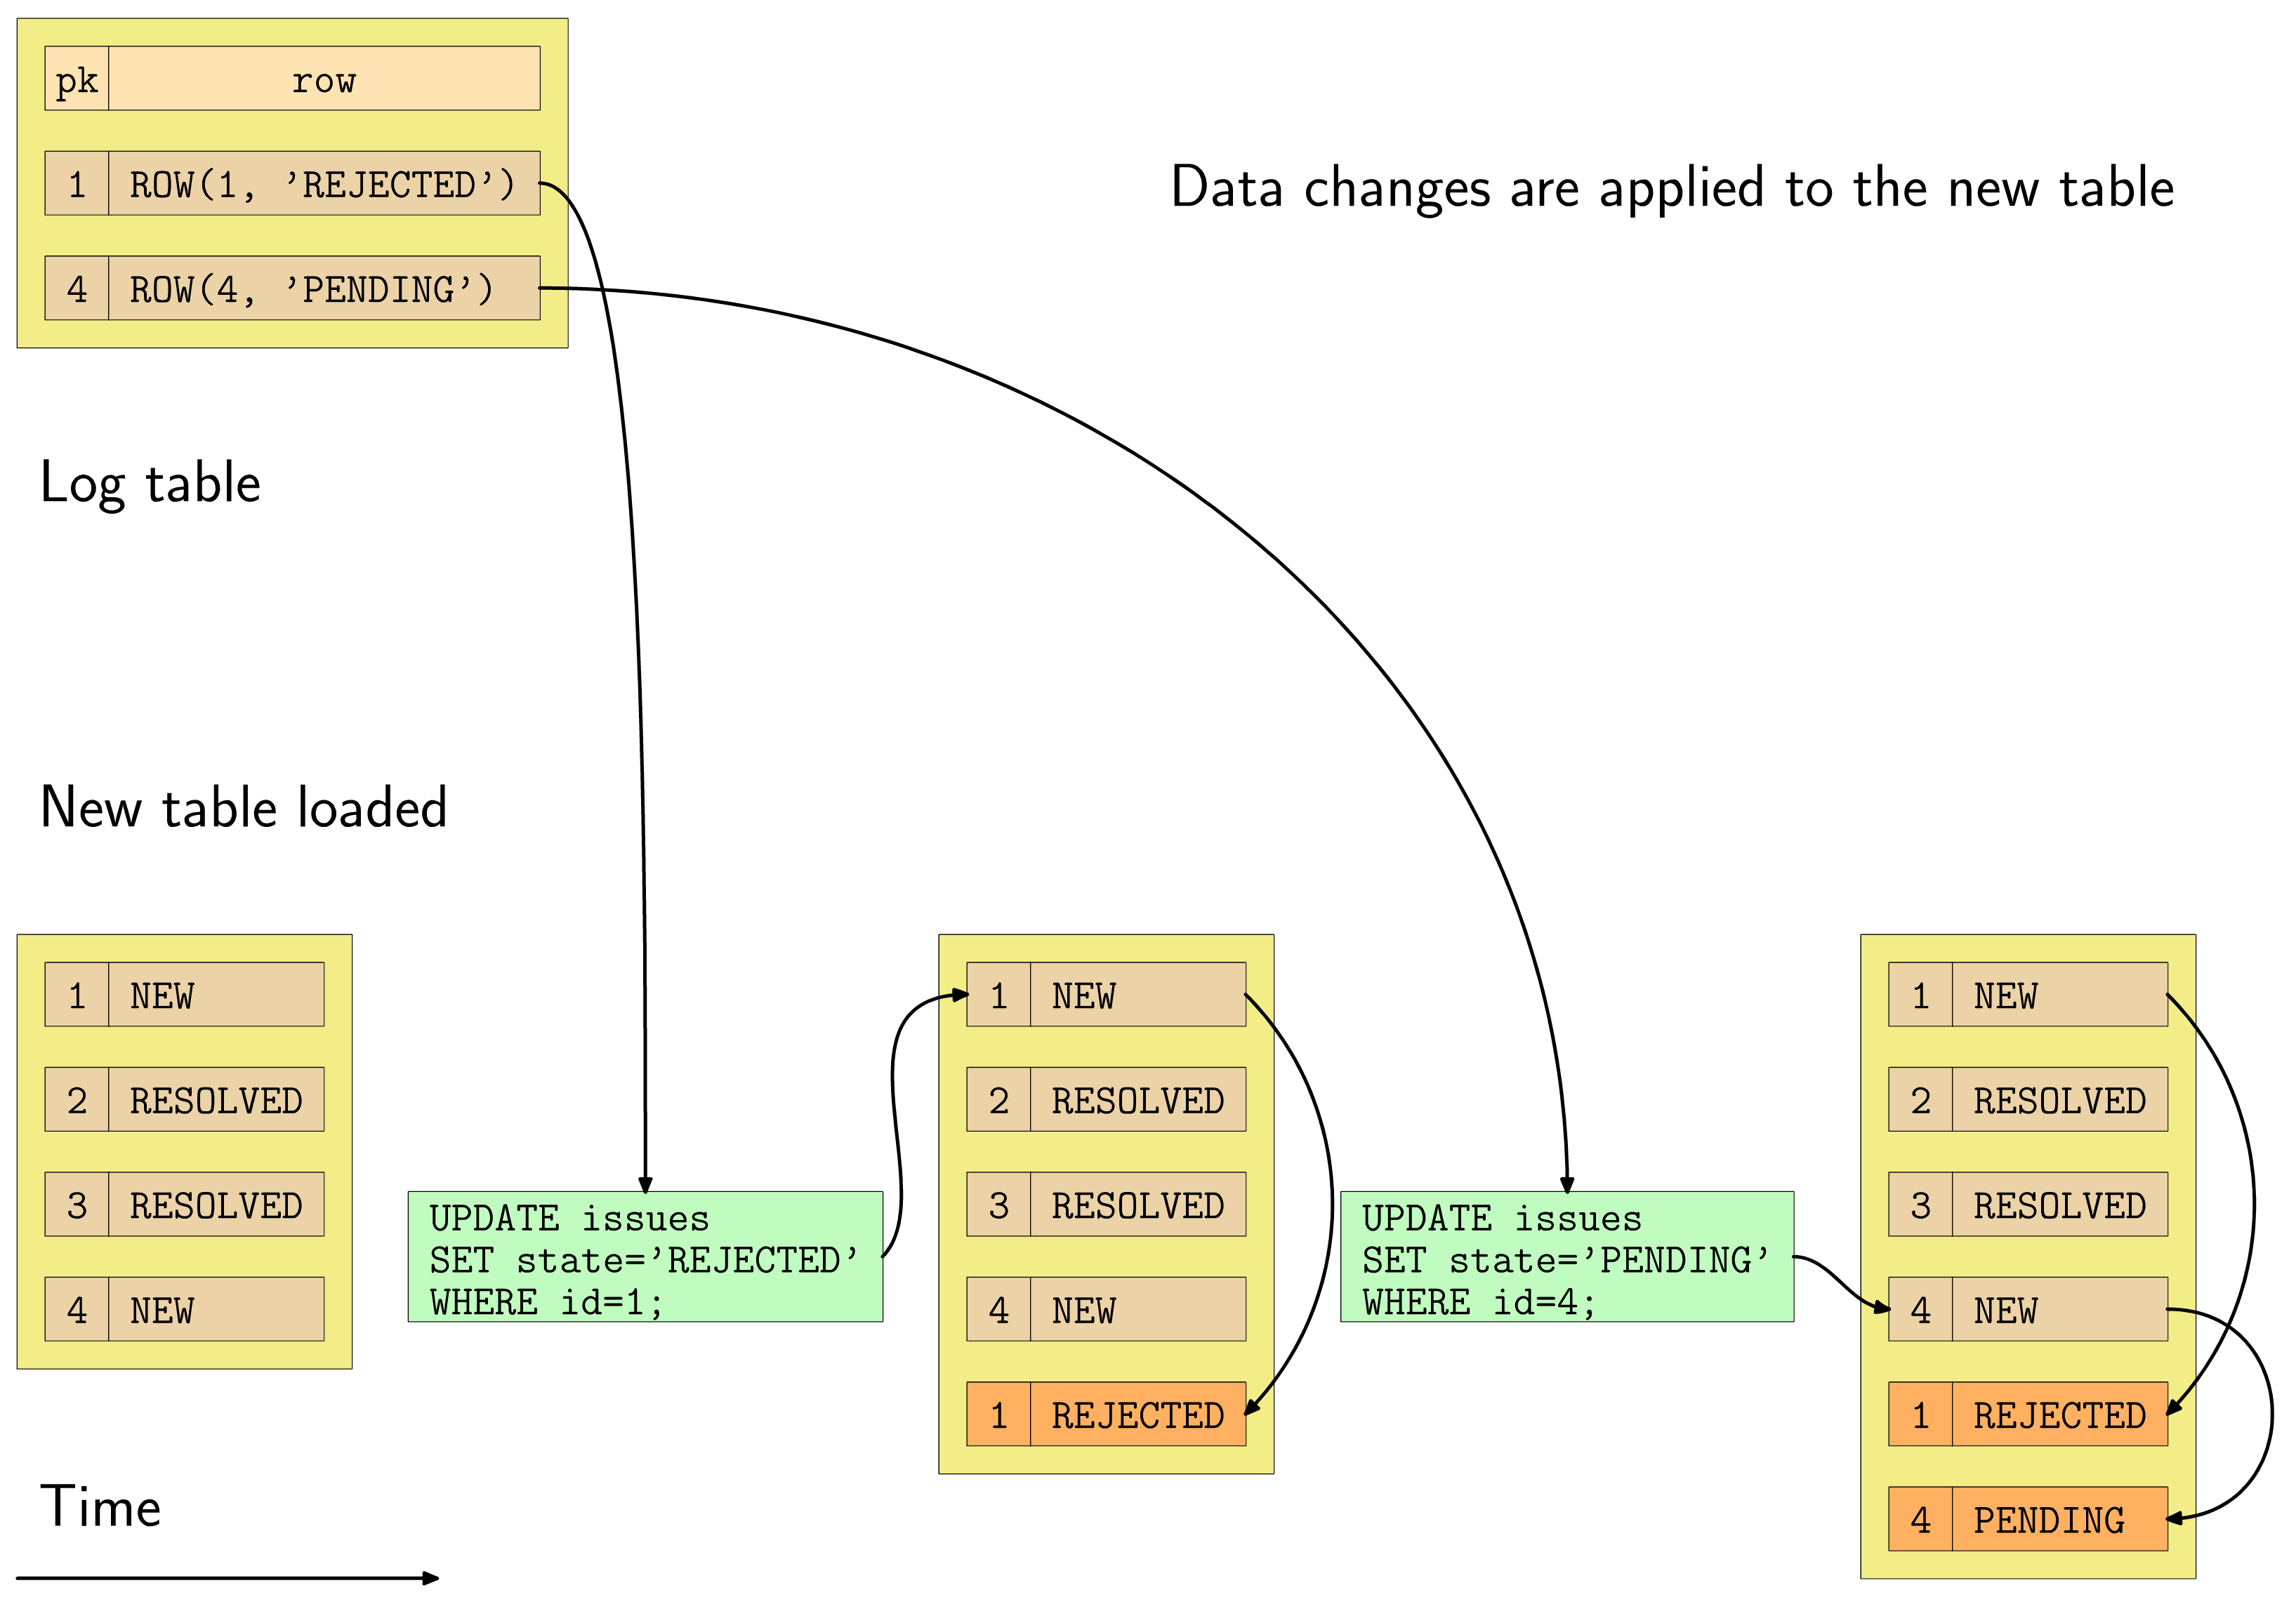
\includegraphics[height=\sizeforimages\textheight]{images/pg_repack_02.png}
  \end{center}
\end{frame}

\begin{frame}
  \frametitle{\texttt{pg\_repack}'s algorithm}
  \begin{itemize}
    \item Like VACUUM FULL / CLUSTER it removes the bloat by copying the
      useful data to a new table, swaps the files and drops the new
      table.
    \item Exclusive lock is held during the swap, but possibly a bit longer if
      the database is too busy.
    \item Data changes done by applications during the copying are captured by
      triggers and written to a ``log table''. They are applied right before
      the swap. (After the initial copying and rebuild of indexes has
      completed.)
      %% TODO Does this line fit to this slide, or should one slide be added?
    \item Multiple backends can be launched to rebuild indexes
  \end{itemize}
\end{frame}

\begin{frame}
  \frametitle{\texttt{pg\_squeeze}}
  \begin{itemize}
    \item Started in 2016 (PostgreSQL 9.5)
    \item The idea was to use background worker to launch \texttt{pg\_repack} automatically
    \item \texttt{pg\_repack} is implemented both on server and client side --
      not really suitable for background worker
  \end{itemize}
\end{frame}

\begin{frame}
  \frametitle{\texttt{pg\_squeeze}}
  \begin{center}
    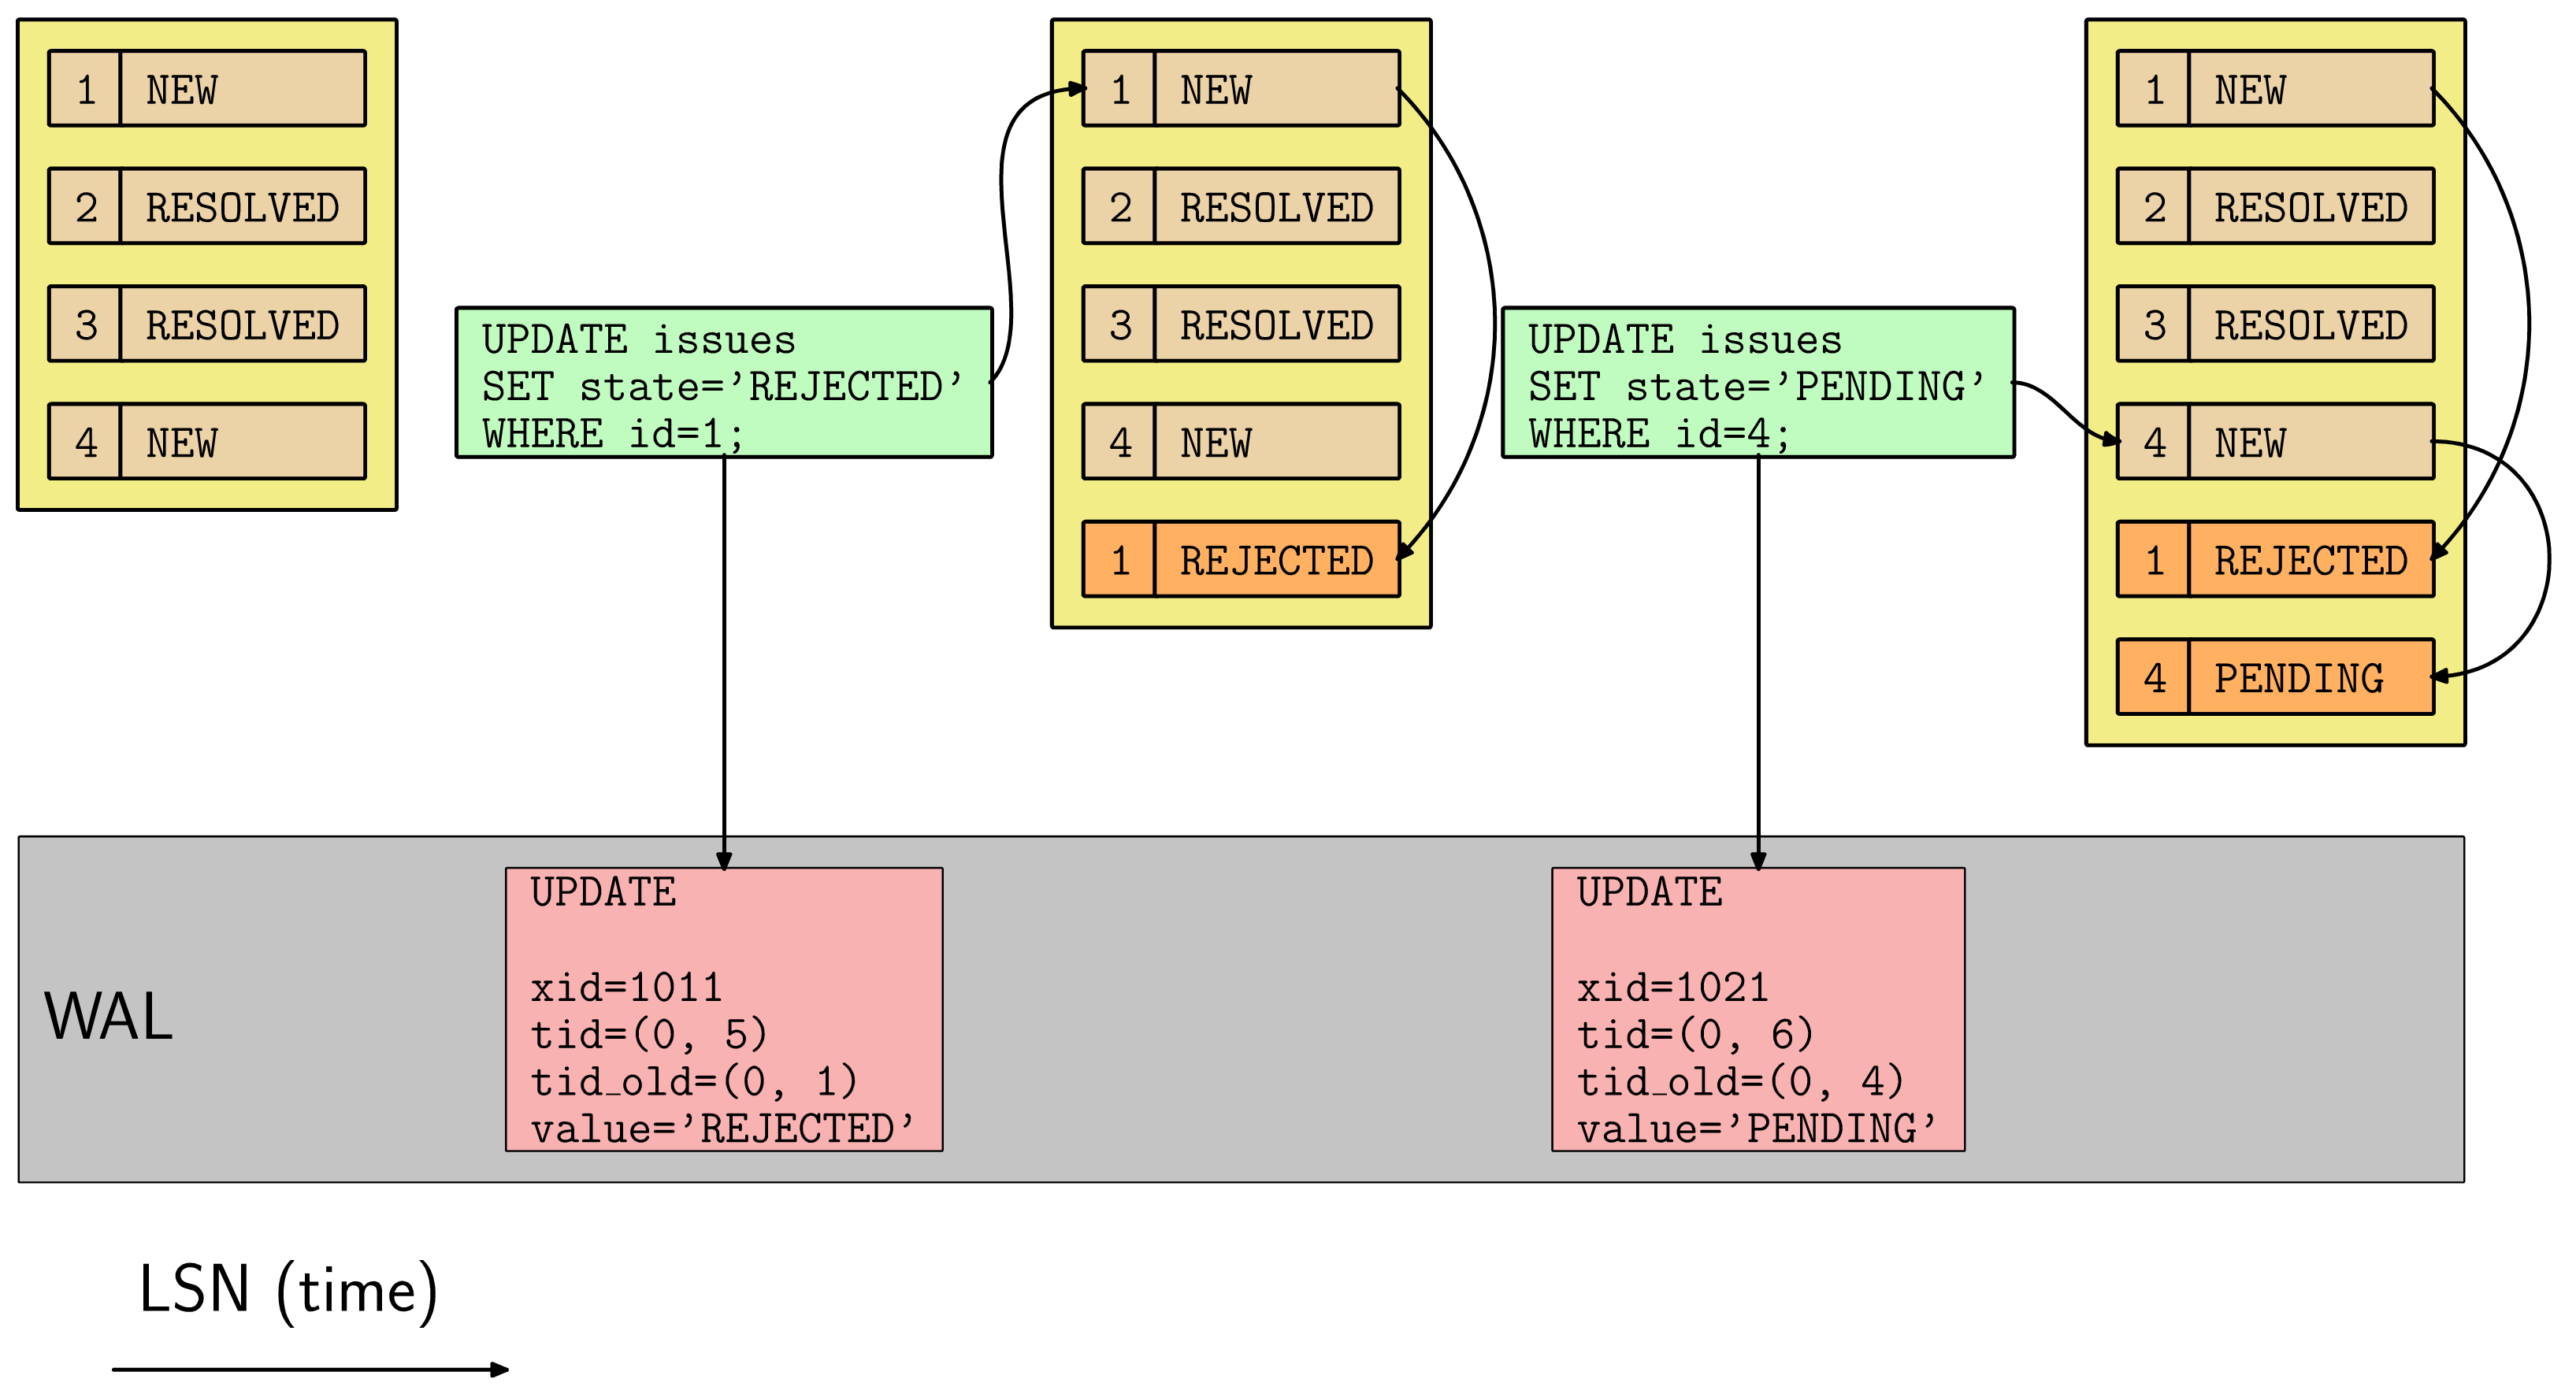
\includegraphics[height=\sizeforimages\textheight]{images/pg_squeeze_01.png}
  \end{center}
\end{frame}

\begin{frame}
  \frametitle{\texttt{pg\_squeeze}}
  \begin{center}
    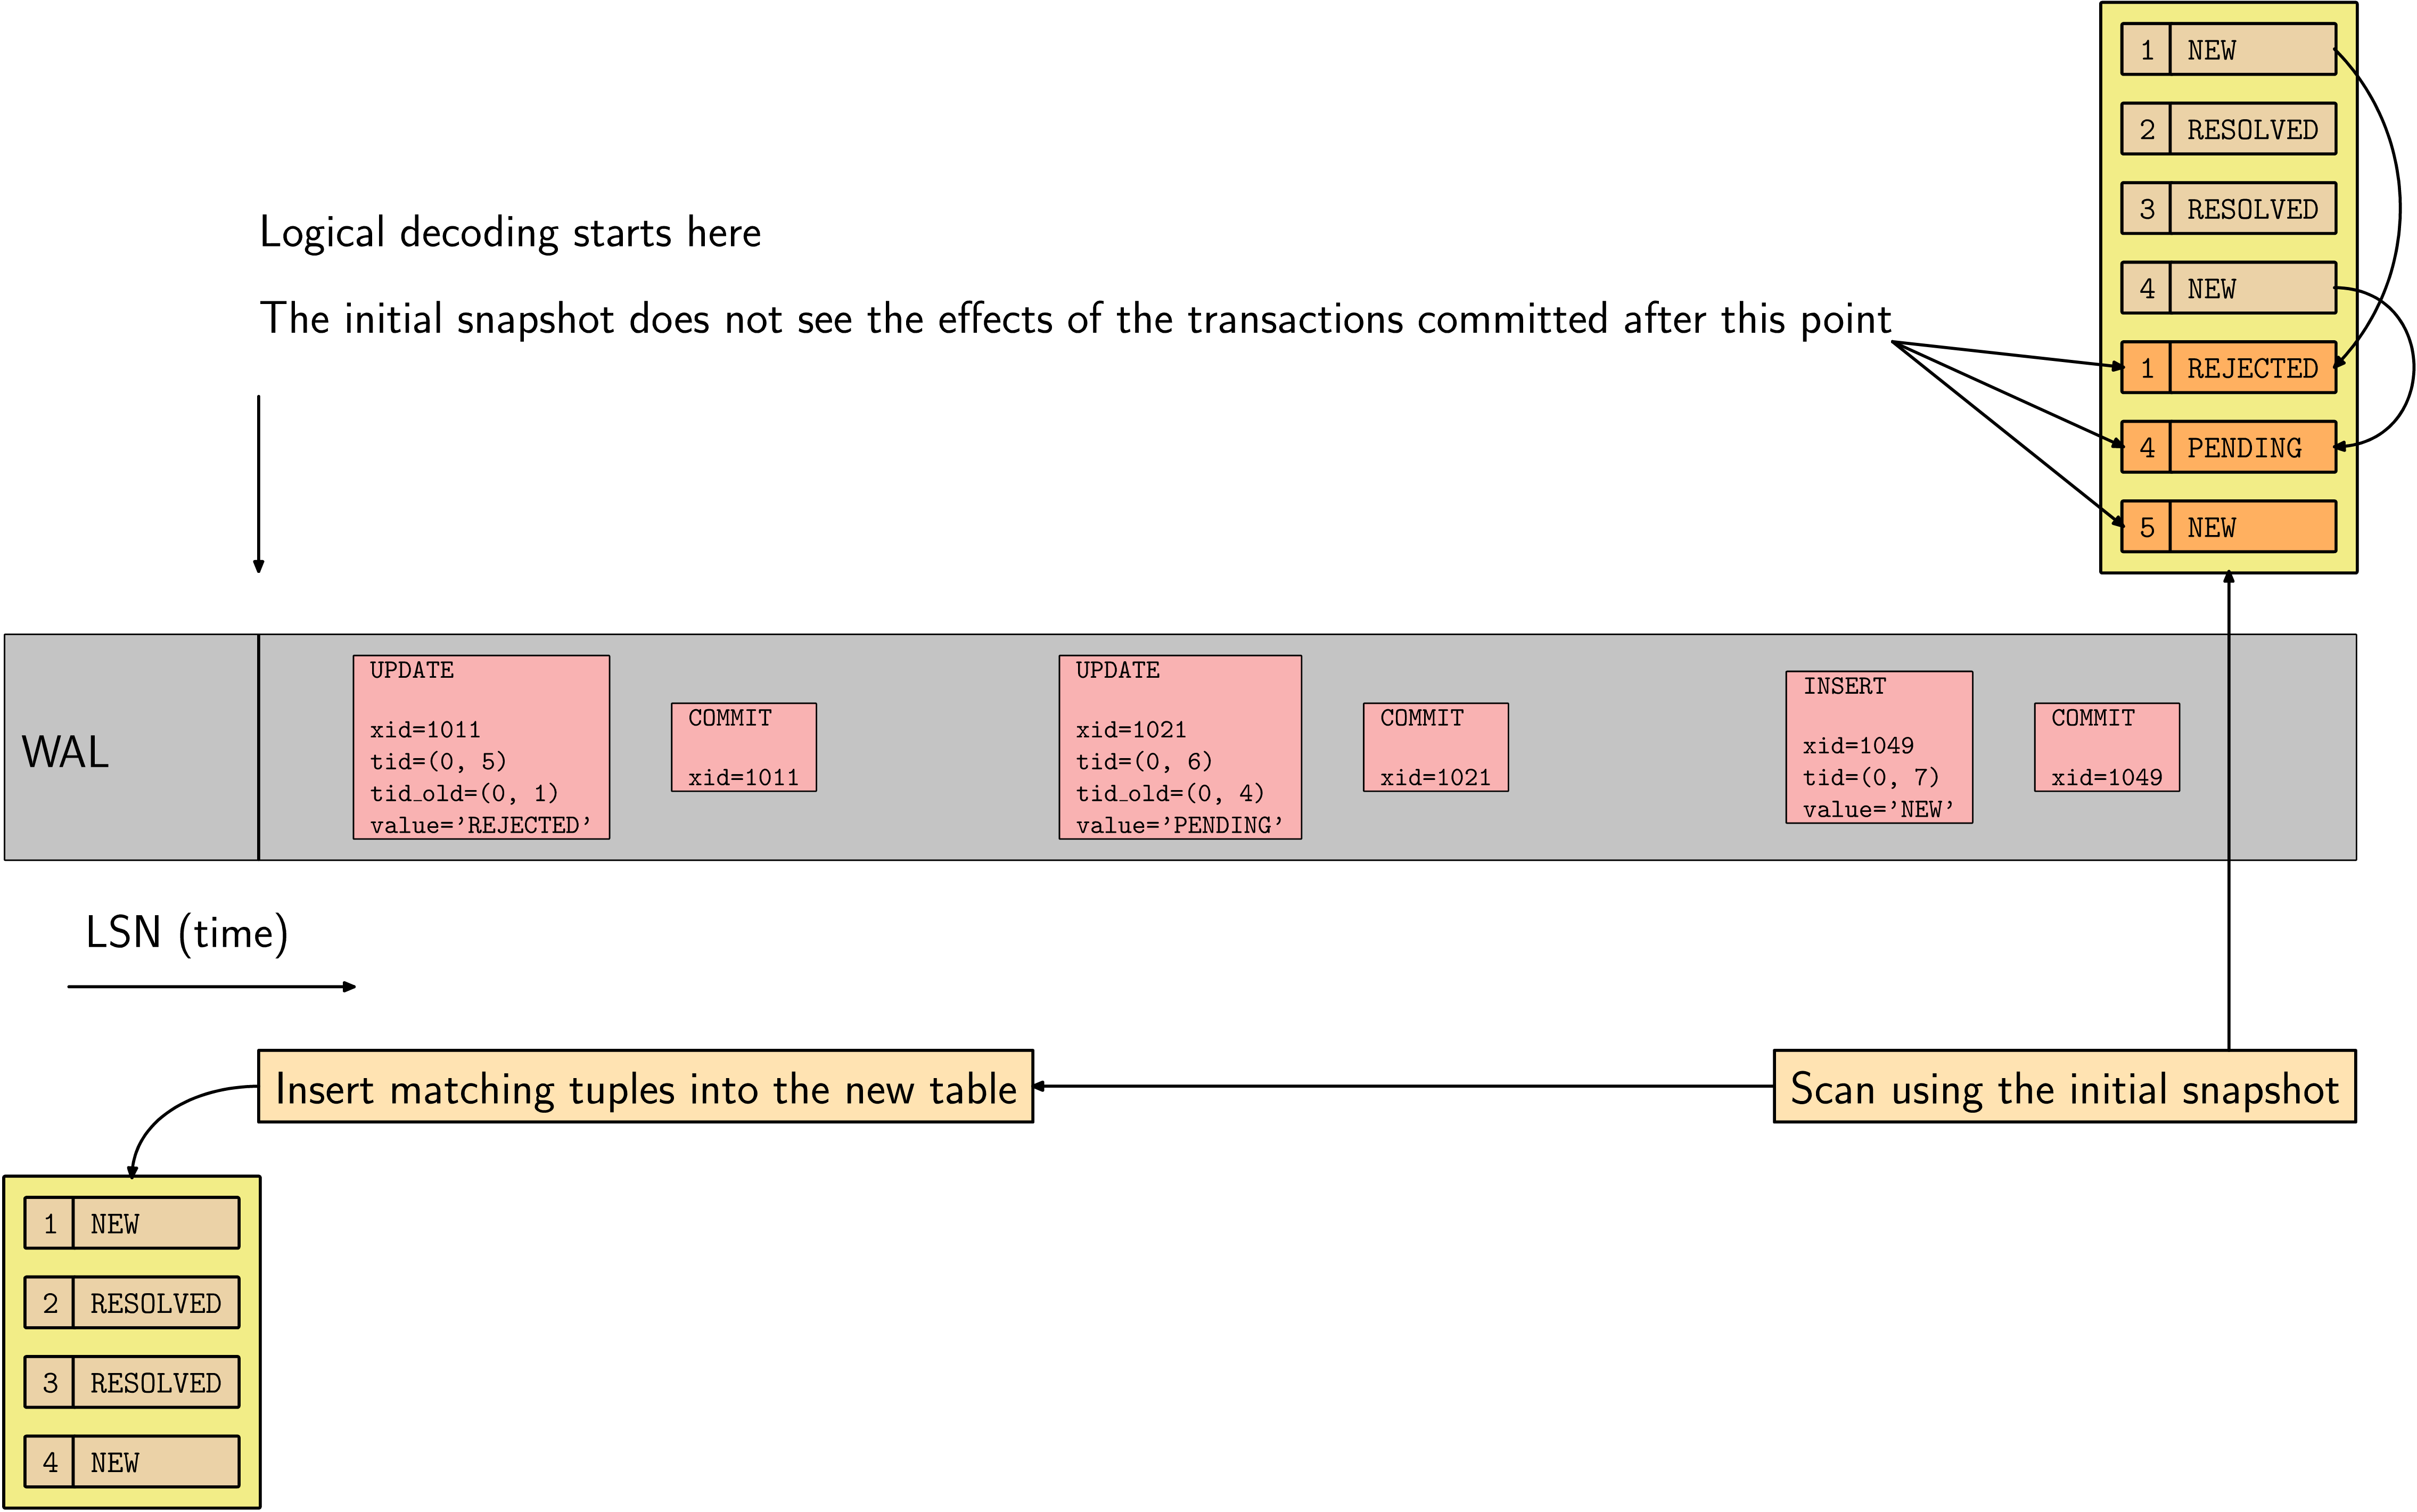
\includegraphics[height=\sizeforimages\textheight]{images/pg_squeeze_02.png}
  \end{center}
\end{frame}

\begin{frame}
  \frametitle{\texttt{pg\_squeeze}}
  \begin{center}
    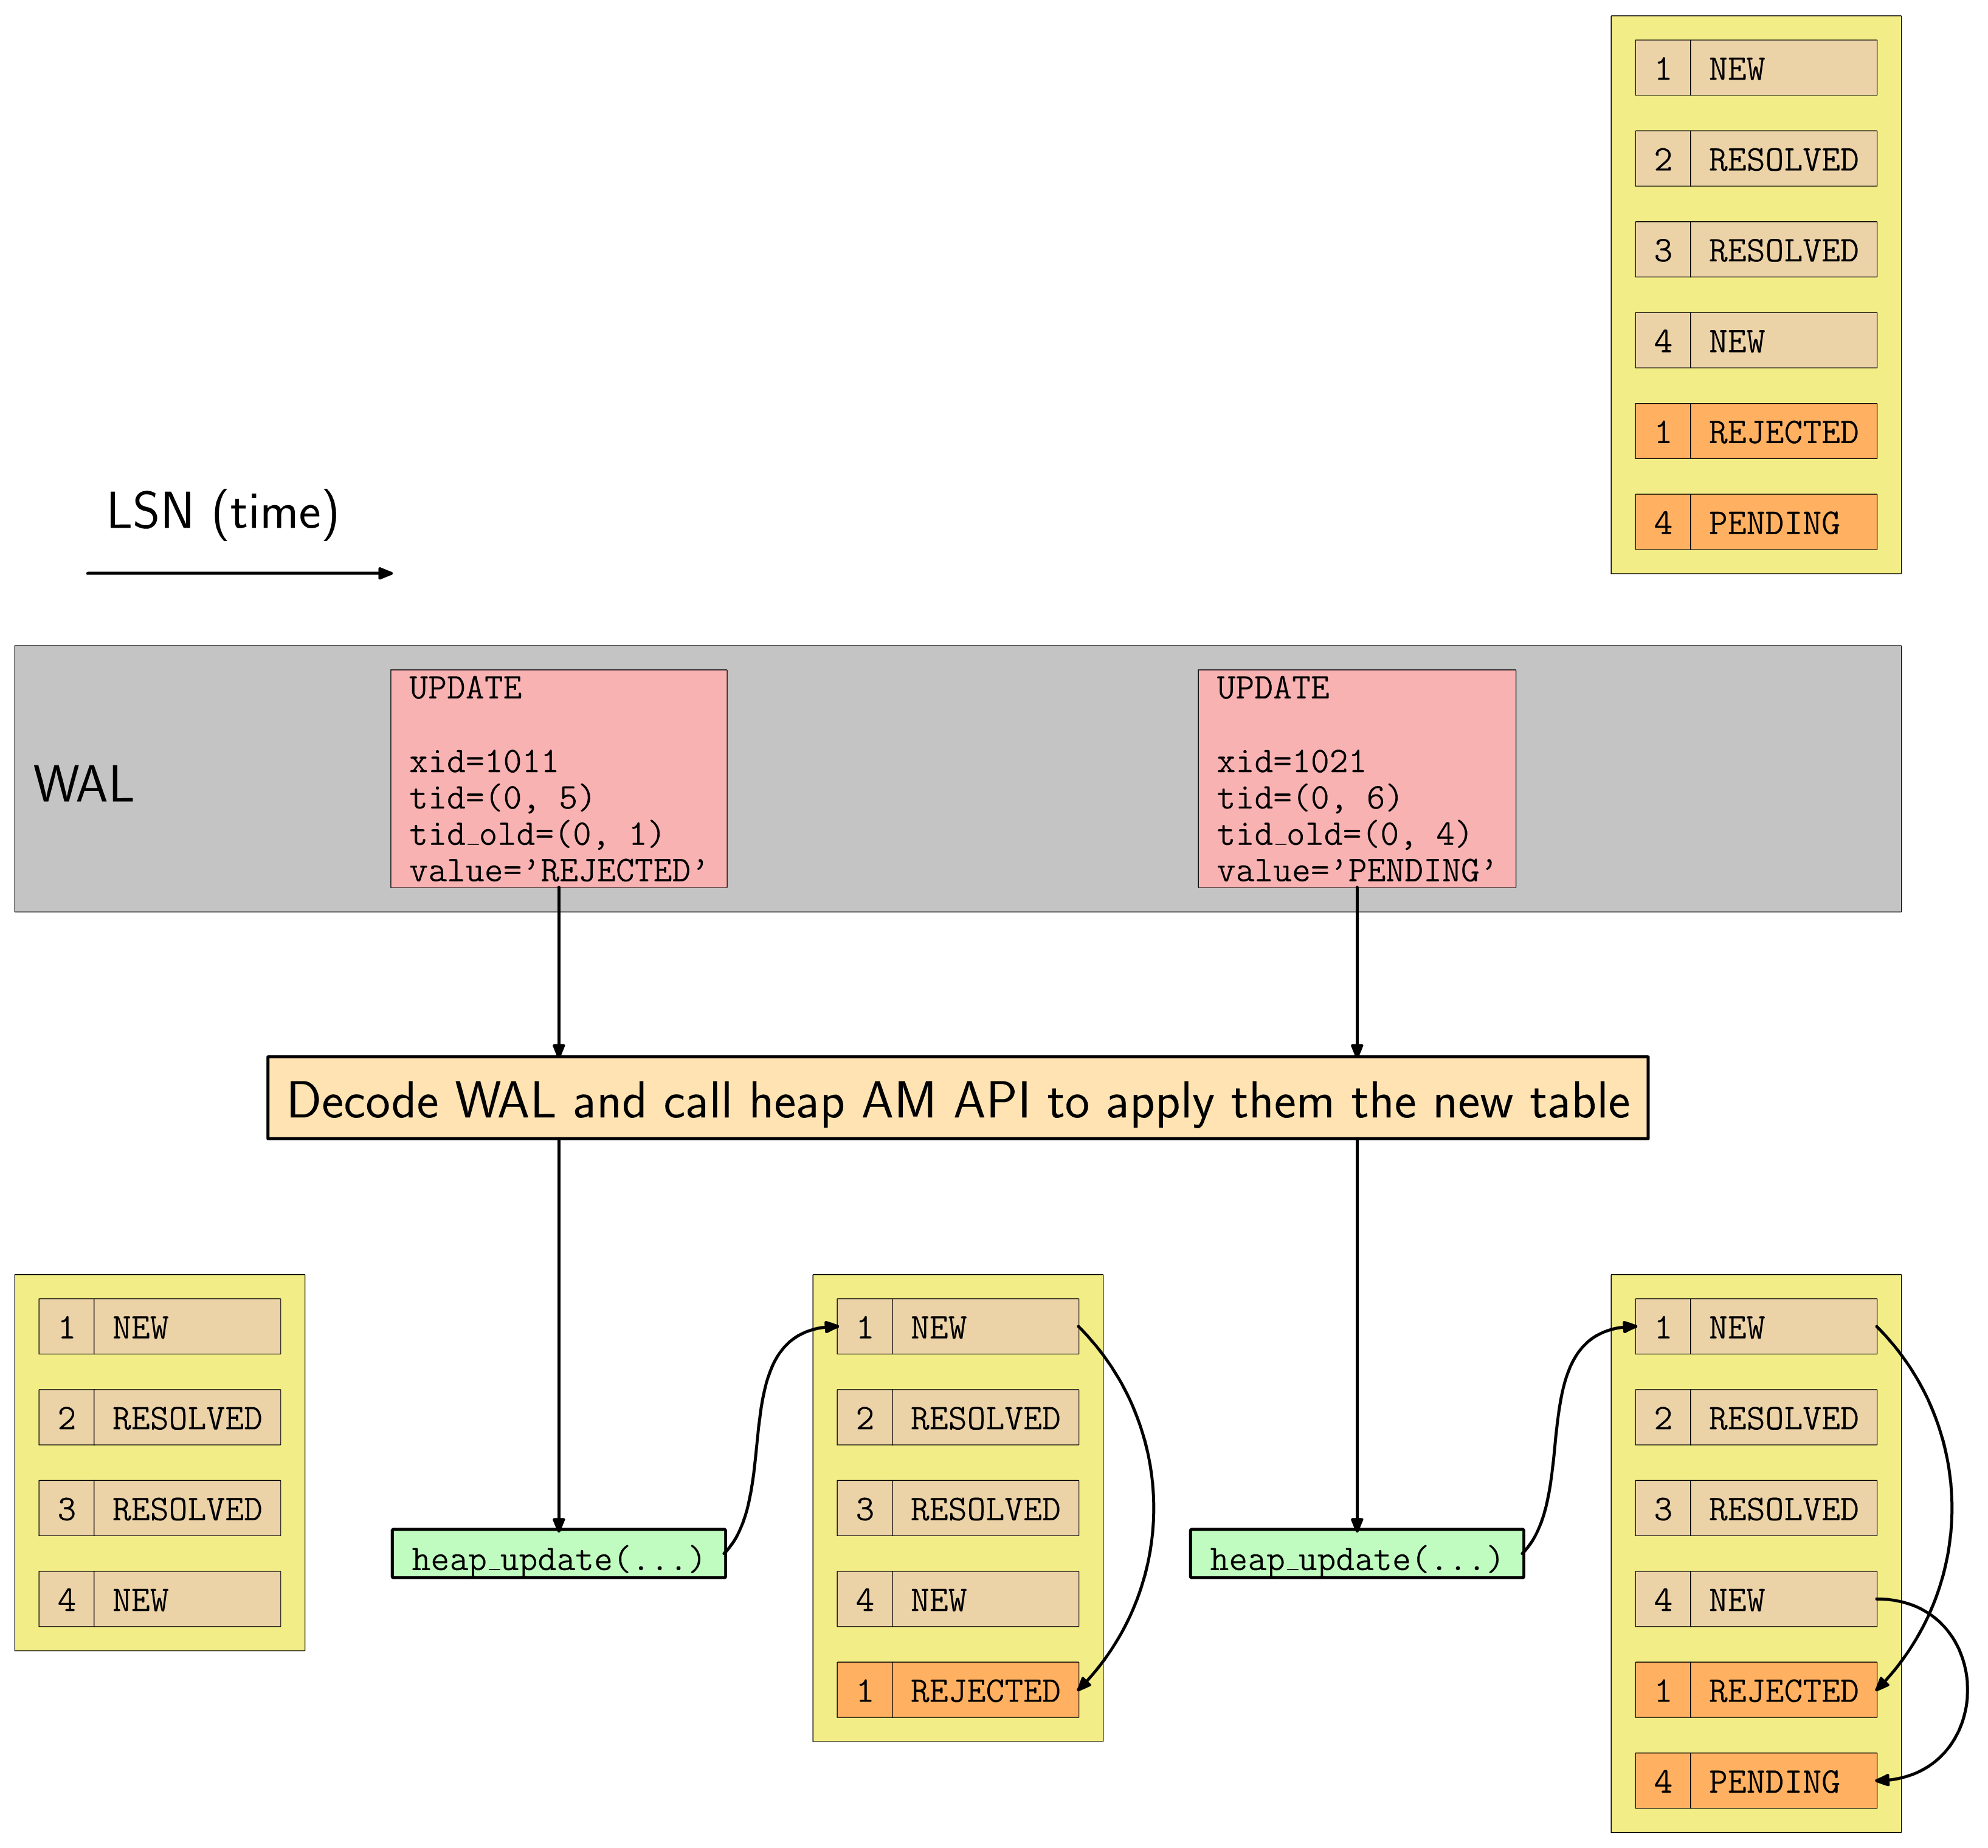
\includegraphics[height=\sizeforimages\textheight]{images/pg_squeeze_03.png}
  \end{center}
\end{frame}

\begin{frame}
  \frametitle{\texttt{pg\_squeeze}}
  \begin{itemize}
    \item Use logical decoding (introduced in PostgreSQL 9.4) rather than
      triggers.
    \item Use server API rather than SQL commands to manipulate tables,
      indexes and data.
    \item Work with binary data rather then text.
    \item cron-like scheduling. Squeeze table if the portion of bloat exceeded
      threshold specified by the DBA.
  \end{itemize}
\end{frame}


%% TODO 1. Disk space requirements, 2. GUC for maximum lock time (probably not
%% used much)
%% \begin{frame}
%%         \frametitle{\texttt{pg\_squeeze}}
%\end{frame}

\section{Repacking done right}
\begin{frame}
  \frametitle{The REPACK command}
  \begin{itemize}
    \item \texttt{REPACK} subsumes \texttt{CLUSTER} and \texttt{VACUUM FULL}
  \end{itemize}
  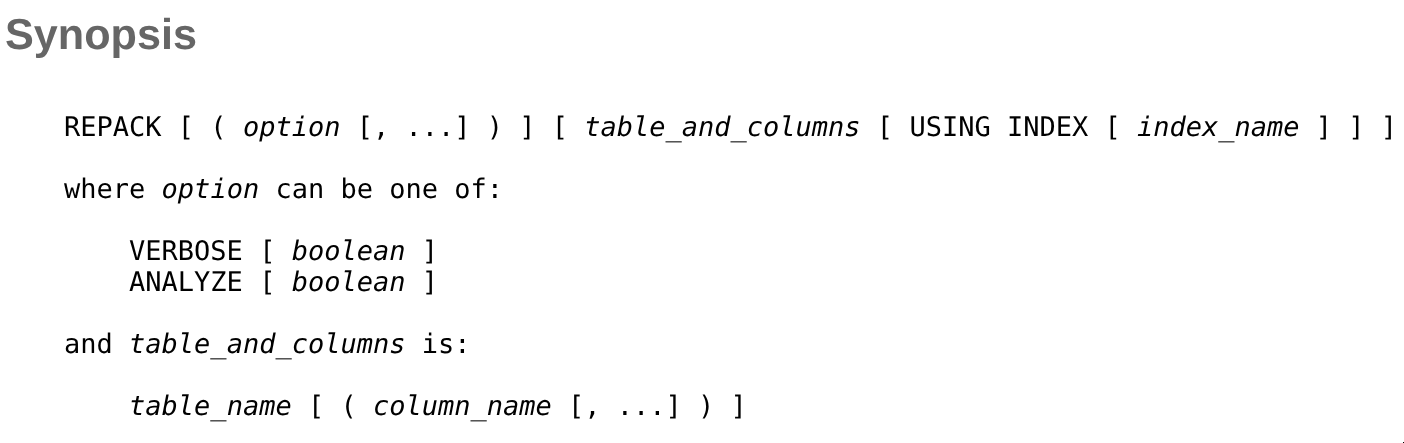
\includegraphics[width=\textwidth]{repack.png}
\end{frame}

\begin{frame}
  \frametitle{Single-table \texttt{REPACK} forms}
  \begin{itemize}
    \item single-table \texttt{vacuum full}: \\
      \texttt{REPACK (ANALYZE) customers;}
    \item single-table \texttt{cluster}: \\
      \texttt{REPACK (ANALYZE) customers USING INDEX cust\_pkey;}
    \item single-table \texttt{cluster} using the stored index: \\
      \texttt{REPACK (ANALYZE) customers USING INDEX;}
  \end{itemize}
\end{frame}

\begin{frame}
  \frametitle{Full-database \texttt{REPACK} forms}
  \begin{itemize}
    \item whole-database \texttt{VACUUM FULL}: \\
      \texttt{REPACK;}
    \item whole-database \texttt{CLUSTER}: \\
      \texttt{REPACK USING INDEX;}
  \end{itemize}
\end{frame}

\begin{frame}
  \frametitle{REPACK CONCURRENTLY}
  \begin{itemize}
    \item This behaves similar to \texttt{pg\_squeeze}
    \item Differences of note are:
      \begin{itemize}
        \item Does not unlock the table before requesting the exclusive lock.
        \item Should not restrict VACUUM of other tables (problem of ``xmin
          horizon``)
        \item Should not require {\tt wal\_level=logical}
        \item No scheduling - do we need that in the core?
        \item MVCC safety (probably not in PG 19)
        \item Use background worker for decoding? (probably not in PG 19)
      \end{itemize}
  \end{itemize}

% TODO (if there's enough time) Explain differences between pg_squeeze and
% REPACK CONCURRENTLY.
%
% 1. pg_squeeze uses AccessShareLock and releases it before it requests
% AccessExclusiveLock (for the file swap), in order to avoid deadlock. If the
% table changed in between, the whole processing is aborted. This approach is
% proably overly cautious. In REPACK CONCURRENTLY, we use
% ShareUpdateExclusiveLock and then simply upgrade it to AccessExclusiveLock,
% so we don't have to check for concurrent catalog changes. (The risk of
% deadlock during the lock upgrade is probably low.)
%
% 2. Since REPACK CONCURRENTLY does not release the ShareUpdateExclusiveLock
% until done, and since this lock conflicts with VACUUM, it does not have to
% care about the xmin horizon (Note: setting the slot's xmin to
% InvalidTransactionId is yet to be implemented.) On the other hand,
% pg_squeeze allows for VACUUM most of the time, so has to block the xmin
% horizon until the initial copy is complete.
%
% 2. Unlike extension, the core code can implement MVCC safety. (Although not
% necessarily in PG 19).
%
% 3. REPACK does not implement scheduling - not sure it's necessary,
% extensions can do that.
\end{frame}

\begin{frame}
  \frametitle{\texttt{pg\_repackdb}}

    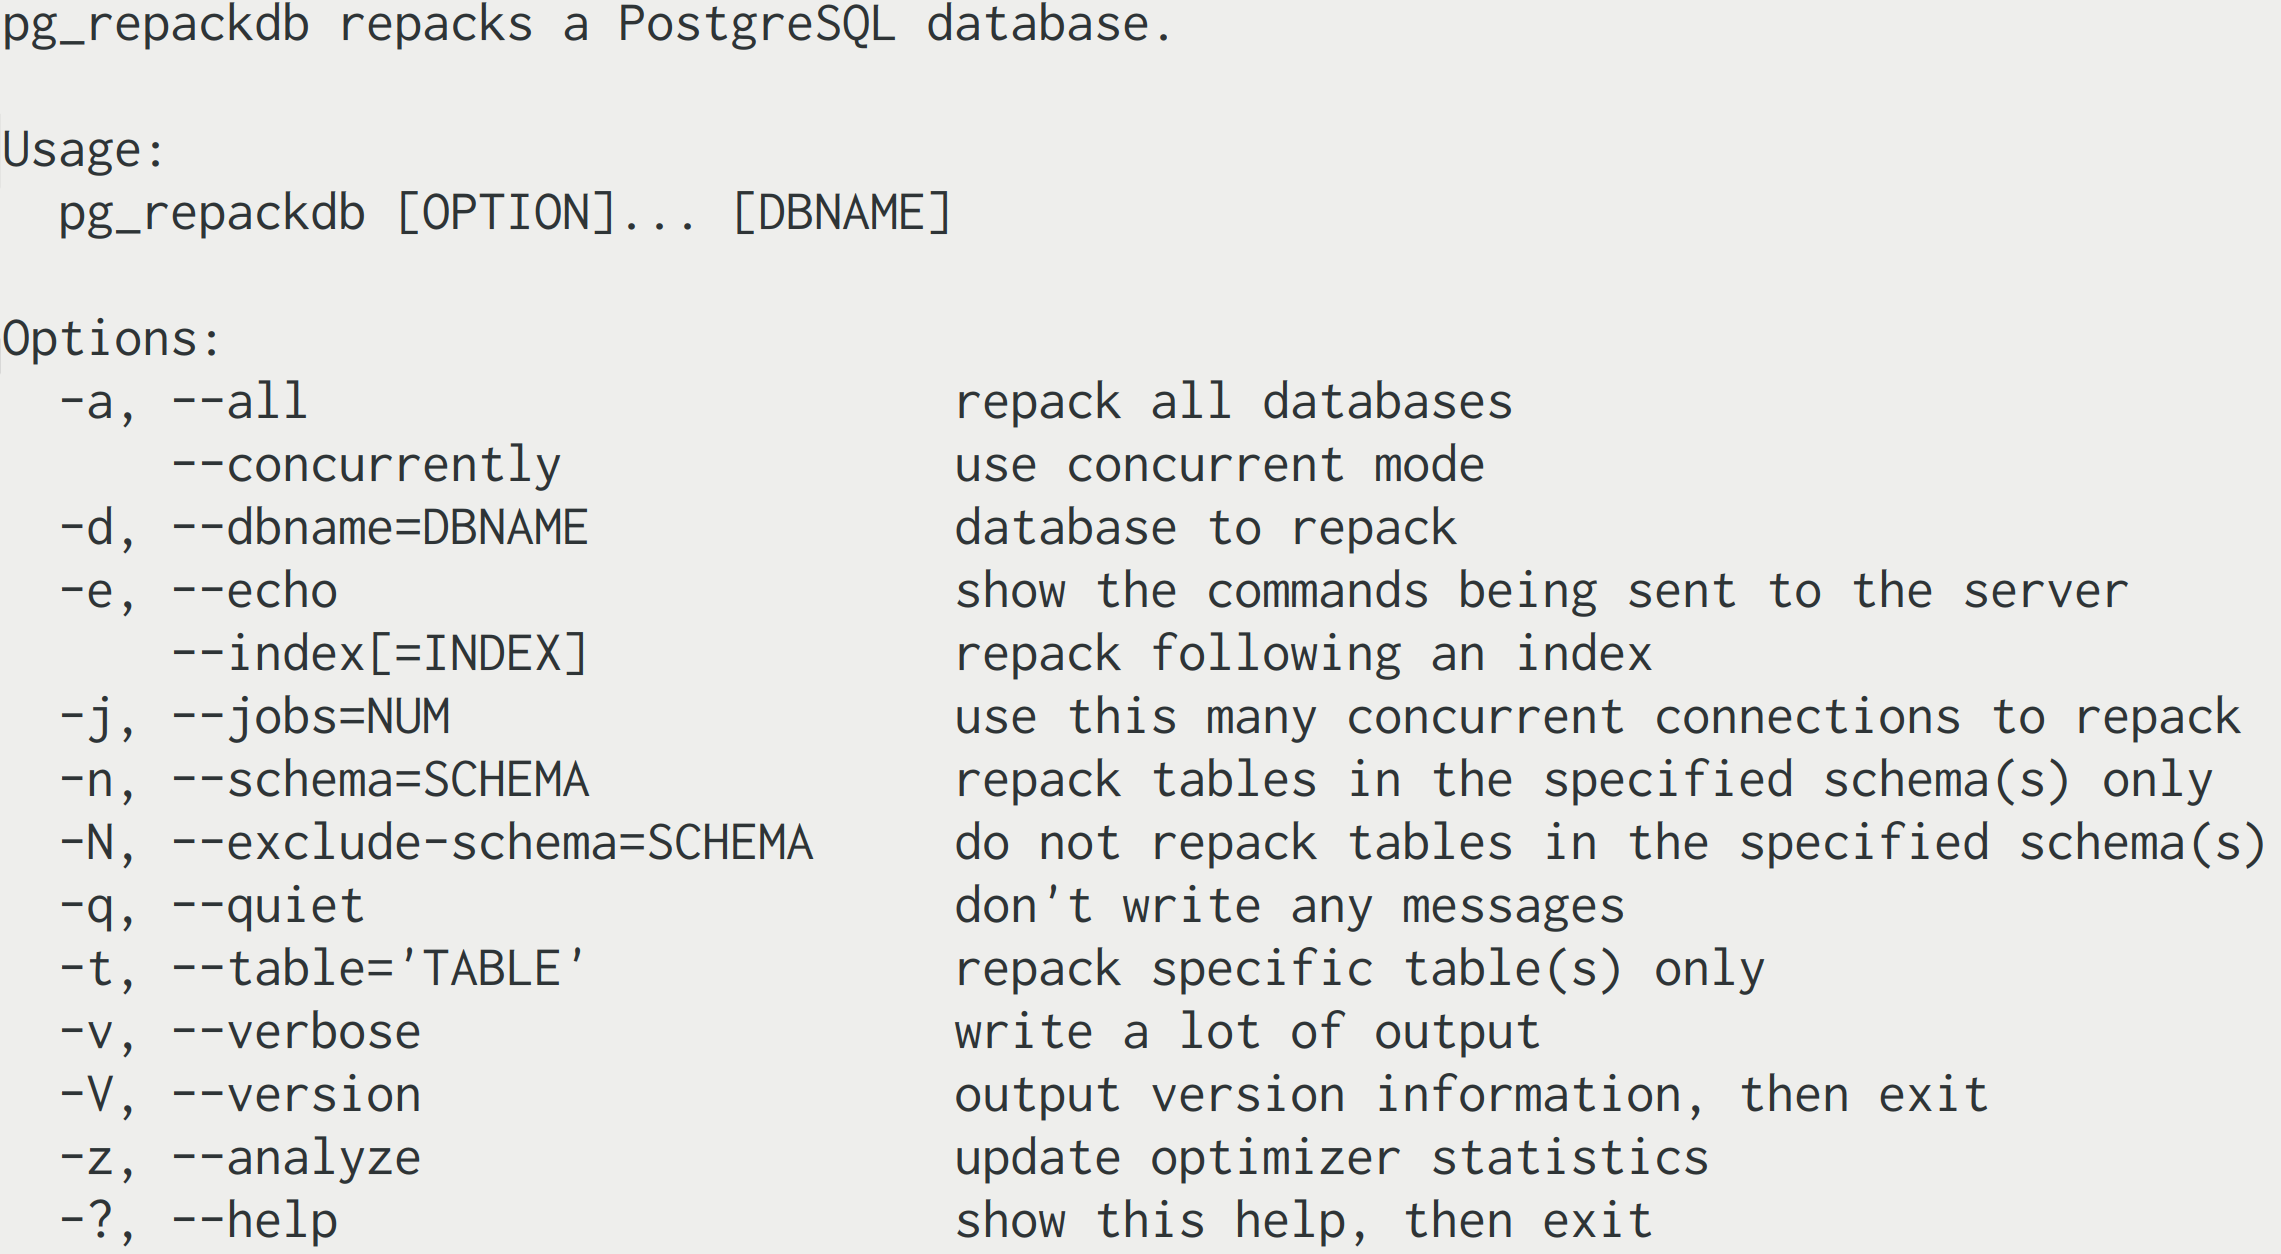
\includegraphics[height=\sizeforimages\textheight]{repackdb.png}
\end{frame}

\section{Future work}

\begin{frame}
  \frametitle{Future work}
  \begin{itemize}
    \item allow to enable logical decoding on the fly
    \item use a background worker for logical decoding
    \item MVCC safety?
    \item Better control over repacking multiple tables?
  \end{itemize}
\end{frame}
